% Edit by: Xiao Xing
% !TEX root = ./main.tex
\setcounter{chapter}{3}

\chapter{大数定律与中心极限定理\label{cha:4}}
大数定律与中心极限定理

\section{特征函数}

设 $ p (x) $ 是随机变量 $ X $ 的密度函数,
则 $ p (x) $ 的傅里叶变换是
\begin{equation*}
    \varphi (t) = \int_{-\infty}^{+\infty} \ee^{itx} p (x) \dd x,
\end{equation*}
其中 $ i = \sqrt{-1} $ 是虚数单位.
由数学期望的概念知,
$ \varphi (t) $ 恰好是 $ E \bigl( \ee^{itx} \bigr) $.
这就是本节要讨论的特征函数,
它是处理许多概率论问题的有力工具,
它能把寻求独立随机变量和的分布的卷积运算 (积分运算) 转换成乘法运算,
还能把求分布的各阶原点矩 (积分运算) 转换成微分运算.
特别它能把寻求随机变量序列的极限分布转换成一般的函数极限问题,
下面从特征函数的定义开始介绍它们.

\subsection{特征函数的定义}

\begin{definition}{}{4.1.1}
    设 $ X $ 是一个随机变量,
    称
    \begin{equation}\label{eq:4.1.1}
        \varphi (t) = E \bigl( \ee^{itx} \bigr), \; -\infty \leq t \leq +\infty,
    \end{equation}
    为 $ X $ 的{\heiti 特征函数}\index{特征函数}.
\end{definition}

因为 $ \lvert \ee^{itx} \rvert \leq 1 $,
所以 $ E \bigl( \ee^{itX} \bigr) $ 总是存在的,
即任一随机变量的特征函数总是存在的.

当离散随机变量 $ X $ 的分布列为 $ p_k = P ( X = x_k ) $, $ k = 1,2,\dotsc $,
则 $ X $ 的特征函数为
\begin{equation}\label{eq:4.1.2}
    \varphi (t) = \sum_{k=1}^{+\infty} \ee^{itx_k} p_k, \; -\infty \leq t \leq +\infty.
\end{equation}

当连续随机变量 $ X $ 的密度函数为 $ p (x) $,
则 $ X $ 的特征函数为
\begin{equation}\label{eq:4.1.3}
    \varphi (t) = \int_{-\infty}^{+\infty} \ee^{itx} p (x) \dd x, \; -\infty \leq t \leq +\infty.
\end{equation}

与随机变量的数学期望、方差及各阶矩一样,
特征函数只依赖于随机变量的分布,
分布相同则特征函数也相同,
所以我们也常称为某{\heiti 分布的特征函数}\index{特征函数!分布的特征函数}.


\begin{example}\label{exam:4.1.1}
    常用分布的特征函数
    \begin{enumerate}
        \item
        {\heiti 单点分布}\index{分布!单点分布}: $ P (X = a) = 1 $,
        其特征函数为
        \begin{equation*}
            \varphi (t) = \ee^{itz}.
        \end{equation*}
        \item\label{exam:4.1.1.2}
        {\heiti 0-1分布}\index{分布!0-1分布}: $ P( X = x ) = p^x  ( 1 - p )^{1 - x} $, $ x = 0,1 $,
        其特征函数为
        \begin{equation*}
            \varphi (t) = p \ee^{it} + q, \quad \text{其中} \ q= 1 - p.
        \end{equation*}
        \item
        {\heiti 泊松分布}\index{分布!泊松分布}: $ P ( X = k ) = ( \lambda^k/k! ) \ee^{-\lambda} $, $ k = 0, 1, \dotsc $, 其特征函数为
        \begin{equation*}
            \varphi (t) = \sum_{k=0}^{+\infty} \ee^{ikt} \frac{\lambda^k}{k!} \ee^{-\lambda} = \ee^{\lambda} \ee^{\lambda \ee^{it}} = \ee^{\lambda ( \ee^{it} ) -1}.
        \end{equation*}
        \item
        {\heiti 均匀分布}\index{分布!均匀分布} $ U ( a,b ) $: 因为密度函数为
        \begin{equation*}
            p (x) =
            \begin{cases}
                \dfrac{1}{b-a}, & a < x < b,\\
                0, & \text{其他}.
            \end{cases}
        \end{equation*}
        所以特征函数为
        \begin{equation*}
            \varphi (t) = \int_a^b \frac{\ee^{itx}}{b - a} \dd x = \frac{\ee^{ibt} - \ee^{iat}}{it (b-a)}.
        \end{equation*}
        \item
        {\heiti 标准正态分布}\index{分布!标准正态分布} $ N (0,1) $: 因为密度函数为
        \begin{equation*}
            p (x) = \frac{1}{\sqrt{2\pi}} \exp \left( -\frac{x^2}{2} \right), \quad - \infty < x < + \infty.
        \end{equation*}
        所以特征函数为
        \begin{align*}
            \varphi (t) & = \frac{1}{\sqrt{2\pi}} \int_{-\infty}^{+\infty} \exp \left( itx - \frac{x^2}{2} \right) \dd x\\
            & = \exp \left( -\frac{t^2}{2} \right) \frac{1}{\sqrt{2\pi}} \int_{-\infty}^{+\infty} \exp \left( -\frac{( x - it )^2}{2} \right) \dd x\\
            & = \exp \left( -\frac{t^2}{2} \right) \frac{1}{\sqrt{2\pi}} \int_{-\infty -it}^{+\infty -it} \exp \left( -\frac{x^2}{2} \right) \dd x\\
            & = \exp \left( -\frac{t^2}{2} \right),
        \end{align*}
        其中
        \begin{equation*}
            \int_{-\infty -it}^{+\infty -it} \exp \left( -\frac{x^2}{2} \right) \dd x = \sqrt{2\pi}
        \end{equation*}
        是利用复变函数中的围道积分求得的.
        有了标准正态分布的特征函数,
        再利用下节给出的特征函数的性质,
        就很容易得到一般正态分布 $ N ( \mu, \sigma^2 ) $ 的特征函数,
        见例~\ref{exam:4.1.2}.
        \item
        {\heiti 指数分布}\index{分布!指数分布} $ Exp ( \lambda ) $: 因为密度函数为
        \begin{equation*}
            p (x) =
            \begin{cases}
                \lambda \ee^{-\lambda x}, & x > 0,\\
                0, & x \leq 0.
            \end{cases}
        \end{equation*}
        所以特征函数为
        \begin{align*}
            \varphi (t) & = \int_0^{+\infty} \ee^{itx} \lambda \ee^{-\lambda x} \dd x\\
            & = \lambda \left( \int_0^{+\infty} \cos (tx) \ee^{-\lambda x} \dd x + i \int_0^{+\infty} \sin (tx) \ee^{-\lambda x} \dd x \right)\\
            & = \lambda \left( \frac{\lambda}{\lambda^2 + t^2} + i \frac{t}{\lambda^2 + t^2} \right)\\
            & = \left( 1 - \frac{it}{\lambda} \right)^{-1}.
        \end{align*}
        以上积分中用到了复变函数中的欧拉公式: $ \ee^{itx} = \cos (tx) + i \sin ( tx) $.
    \end{enumerate}
\end{example}

\subsection{特征函数的性质}

现在我们来研究特征函数的一些性质,
其中 $ \varphi_X (t) $ 表示 $ X $ 的特征函数,
其他类似.

\begin{property}\label{prop:4.1.1}
    \begin{equation}\label{eq:4.1.4}
        \lvert \varphi (t) \rvert \leq \varphi (0) = 1.
    \end{equation}
\end{property}

\begin{property}\label{prop:4.1.2}
    \begin{equation}\label{eq:4.1.5}
        \varphi (-t) = \overline{\varphi (t)},
    \end{equation}
    其中 $ \overline{\varphi (t)} $ 表示 $ \varphi (t) $ 的共轭.
\end{property}

\begin{property}\label{prop:4.1.3}
    若 $ Y = aX + b $, 其中 $ a,b $ 是常数, 则
    \begin{equation}\label{eq:4.1.6}
        \varphi_Y (t) = \ee^{ibt} \varphi_X (at).
    \end{equation}
\end{property}

\begin{property}\label{prop:4.1.4}
    独立随机变量和的特征函数为特征函数的积,
    即设 $ X $ 与 $ Y $ 相互独立, 则
    \begin{equation}\label{eq:4.1.7}
        \varphi_{X+Y} (t) = \varphi_X (t) \cdot \varphi_Y (t).
    \end{equation}
\end{property}

\begin{property}\label{prop:4.1.5}
    若 $ E (x^l) $ 存在,
    则 $ X $ 的特征函数 $ \varphi(t) $ 可 $ l $ 次求导,
    且对 $ 1 \leq k \leq l $, 有
    \begin{equation}\label{eq:4.1.8}
        \varphi^{(k)} (0) = i^k E ( X^k ).
    \end{equation}
    上式提供了一条求随机变量的各阶矩的途径,
    特别可用下式去求数学期望和方差.
    \begin{equation}\label{eq:4.1.9}
        E (X) = \frac{\varphi' (0)}{i}, \quad \mathrm{Var} (X) = - \varphi'' (0) + \bigl( \varphi' (0) \bigr)^2.
    \end{equation}
\end{property}

\begin{proof}
    在此我们仅对连续场合进行证明,
    而在离散场合的证明是类似的.
    \begin{enumerate}
        \item
        \begin{align*}
            \lvert \varphi (t) \rvert & = \left\lvert \int_{-\infty}^{+\infty} \ee^{itx} p (x) \dd x \right\rvert
            \leq \int_{-\infty}^{+\infty} \left\lvert \ee^{itx} \right\rvert p (x) \dd x\\
            & = \int_{-\infty}^{+\infty} p (x) \dd x
            = \varphi (0)
            = 1.
        \end{align*}
        \item
        \begin{equation*}
            \varphi (-t) = \int_{-\infty}^{+\infty} \ee^{-itx} p (x) \dd x
            = \overline{\int_{-\infty}^{+\infty} \ee^{itx} p (x) \dd x}
            = \overline{\varphi (t)}.
        \end{equation*}
        \item
        \begin{equation*}
            \varphi_Y (t) = E ( \ee^{it (aX + b)} )
            = \ee^{ibt} E ( \ee^{iatX} ) = \ee^{ibt} \varphi (at).
        \end{equation*}
        \item
        因为 $ X $ 与 $ Y $ 相互独立, 所以 $ \ee^{itX} $ 与 $ \ee^{itY} $ 也是独立的, 从而有
        \begin{equation*}
            E \left( \ee^{it ( X + Y )} \right) = E \left( \ee^{itX} \ee^{itY} \right) = \varphi_X (t) \cdot \varphi_Y (t).
        \end{equation*}
        \item
        因为 $ E \left( X^l \right) $ 存在, 也就是
        \begin{equation*}
            \int_{-\infty}^{+\infty} \lvert x \rvert^l p (x) \dd x < +\infty,
        \end{equation*}
        于是含参变量 $ t $ 的广义积分 $ \int_{-\infty}^{+\infty} \ee^{itx} p(x) \dd x $ 可以对 $ t $ 求导 $ l $ 次, 于是对 $ 0 \leq k \leq l $, 有
        \begin{equation*}
            \varphi ^{(k)} (t) = \int_{-\infty}^{+\infty} i^k x^k \ee^{itx} p (x) \dd x = i^k E \left( X^k \ee^{itX} \right).
        \end{equation*}
        令 $ t = 0 $ 即得
        \begin{equation*}
            \varphi^{(k)} (0) = i^k E \left( X^k \right).
        \end{equation*}
    \end{enumerate}
    至此上述5条性质全部得证.
\end{proof}

下例是利用 \eqref{eq:4.1.6} 和 \eqref{eq:4.1.7} 来求一些常用分布的特征函数.


\begin{example}\label{exam:4.1.2}
    常用分布的特征函数 (二)

    \begin{enumerate}
        \item
        {\heiti 二项分布}\index{分布!二项分布} $ b (n, p) $: 设 $ Y \sim b (n, p) $, 则 $ Y = X_1 + x_2 + \dotsb X_n $, 其中诸 $ X_i $ 是相互独立同分布的随机变量, 且 $ X_{i} \sim b (1, p) $, 由 例~\ref{exam:4.1.2} \ref{exam:4.1.1.2} 知
        \begin{equation*}
            \varphi_{X_i} (t) = p \ee^{it} + q,
        \end{equation*}
        所以由独立随机变量和的特征函数为特征函数的积, 得
        \begin{equation*}
            \varphi_Y (t) = \left( p \ee^{it} + q \right)^{\pi}
        \end{equation*}
        \item
        {\heiti 正态分布}\index{分布!正态分布} $ N (\mu, \sigma^2) $: 设 $ Y \sim N (\mu, \sigma^2) $, 则 $ X = (Y - \mu) / \sigma \sim N (0, 1) $.
        由例~\ref{exam:4.1.1} 知
        \begin{equation*}
            \varphi_{X} (t) = \exp \left( -\frac{t^2}{2} \right).
        \end{equation*}
        所以由 $ Y = \sigma X + \mu $ 得
        \begin{equation*}
            \varphi_Y (t) = \varphi_{\alpha X + \mu} (t) =\ee^{i \mu t} \varphi_X ( \sigma t ) = \exp \left( i \mu t - \frac{\sigma^2 t^2}{2} \right).
        \end{equation*}
        \item
        {\heiti 伽玛分布}\index{分布!伽玛分布} $ Ga ( n, \lambda ) $: 设 $ Y \sim Ga ( n, \lambda ) $, 则$ Y = X_1 + X_2 + \dotsb + X_n $, 其中 $ X_i $ 独立同分布, 且 $ X_i \sim Exp ( \lambda ) $.
        由例~\ref{exam:4.1.1} 知
        \begin{equation*}
            \varphi_{X_i} (t) = \left( 1 - \frac{it}{\lambda} \right)^{-1}.
        \end{equation*}
        所以由独立随机变量和的特征函数为特征函数的积, 得
        \begin{equation*}
            \varphi_Y (t) = \left( \varphi_{X_i} (t) \right)^n = \left( 1 - \frac{it}{\lambda} \right)^{-n}.
        \end{equation*}
        进一步, 当 $ a $为任一正实数时, 我们可得 $ Ga ( n, \lambda ) $ 分布的特征函数为
        \begin{equation*}
            \varphi(t) = \left( 1 - \frac{it}{\lambda} \right)^{-a}.
        \end{equation*}
        \item
        $ \chi^2 (n) $ {\heiti 分布}\index{分布!chi2分布@$\chi^2 (n) $ 分布}: 因为 $ \chi^2 (n) = Ga ( n/2, 1/2 ) $, 所以 $ \chi^2 (n) $ 分布的特征函数为
        \begin{equation*}
            \varphi (t) = ( 1 - 2it )^{-n/2}.
        \end{equation*}
    \end{enumerate}
\end{example}

上述常用分布的特征函数汇总在表~\ref{tab:4.1.1} 中.

\begin{table}
    \renewcommand{\arraystretch}{1.6}
    \centering
    \caption{常用分布的特征函数}\label{tab:4.1.1}
    \begin{tabular}{>{\centering\arraybackslash}m{0.15\linewidth}>{\centering\arraybackslash}m{0.45\linewidth}>{\centering\arraybackslash}m{0.3\linewidth}}
        \toprule
        分布 & 分布列 $ p_k $ 或分布密度 $ p (x) $ & 特征函数 $ \varphi (t) $\\
        \midrule
        单点分布 & $ P (X = a) = 1 $ & $ \ee^{itz} $\\
        0-1分布 & $ P_k = p^k  q^{1 - k} $, $ k = 0,1 $ & $ p \ee^{it} + q $\\
        二项分布 $ b (n, p) $ & $ p_k = \binom{n}{k} p^k q^{1-k} $, $ k = 0,1,\dotsc,n $ & $ \left( p \ee^{it} + q \right)^{\pi} $\\
        泊松分布 $ P (\lambda) $ & $ P_k = ( \lambda^k/k! ) \ee^{-\lambda} $, $ k = 0, 1, \dotsc $ & $ \ee^{\lambda ( \ee^{it} ) -1} $\\
        均匀分布 $ U (a,b) $ & $ p (x) = 1/(b-a) $, $ a \leq x \leq b $ & $ \dfrac{\ee^{ibt} - \ee^{iat}}{it (b-a)} $\\
        正态分布 $ N (\mu, \sigma^2) $ & $ p (x) = \dfrac{1}{\sqrt{2\pi}\sigma} \exp \left( - \dfrac{( x - \mu )^2}{2 \sigma^2} \right) $ & $ \exp \left( i \mu t - \dfrac{\sigma^2 t^2}{2} \right) $\\
        指数分布 $ Exp ( \lambda ) $ & $ p (x) = \lambda \ee^{-\lambda x} $, $ x > 0 $ & $ \left( 1 - \dfrac{it}{\lambda} \right)^{-1} $\\
        伽玛分布 $ Ga ( a, \lambda ) $ & $ p (x) = \dfrac{\lambda^\alpha}{\Gamma (a)} x^{\alpha - 1} \ee^{-\lambda x} $, $ x \geq 0 $ & $ \left( 1 - \dfrac{it}{\lambda} \right)^{-a} $\\
        $ \chi^2 (n) $ 分布 & $ p (x) = \dfrac{x^{n/2 - 1} \ee^{-x/2}}{\Gamma (n/2) 2^{n/2}} $, $ x > 0 $ & $ ( 1 - 2it )^{-n/2} $\\
        \bottomrule
    \end{tabular}
\end{table}

下例是利用 \eqref{eq:4.1.8} 来求分布的数学期望和方差.

\begin{example}\label{exam:4.1.3}
    试利用特征函数的方法求伽玛分布 $ Ga ( n, \lambda ) $ 的数学期望和方差.
\end{example}

\begin{solution}
    因为伽玛分布 $ Ga ( a, \lambda ) $ 的特征函数及其一、二阶导数为
    \begin{gather*}
        \varphi (t) = \left( 1 - \dfrac{it}{\lambda} \right)^{-a},\\
        \varphi' (t) = \frac{ai}{\lambda} \left( 1 - \frac{it}{\lambda} \right)^{-a-1}, \ \varphi' (0) = \frac{ai}{\lambda},\\
        \varphi'' (t) = \frac{a ( a + 1 ) i^2}{\lambda^2} \left( 1 - \frac{it}{\lambda} \right)^{-a-2}, \ \varphi'' (0) = -\frac{a (a+1)}{\lambda^2},
    \end{gather*}
    所以由 \eqref{eq:4.1.9} 得
    \begin{align*}
        E (X) & = \frac{\varphi' (0)}{i} = \frac{a}{\lambda},\\
       \Var  (X) & = - \varphi'' (0) + \bigl( \varphi' (0) \bigr)^2 = \frac{a (a+1)}{\lambda^2} + \left( \frac{ai}{\lambda} \right)^2\\
        & = \frac{a (a+1)}{\lambda^2} - \frac{a^2}{\lambda^2} = \frac{a}{\lambda^2}.
    \end{align*}
\end{solution}

特征函数还有以下一些优良性质.

\begin{theorem}{一致连续性}{4.1.1}
    随机变量 $ X $ 的特征函数 $ \varphi (t) $ 在 $ ( -\infty, +\infty ) $ 上一致连续.
\end{theorem}

\begin{proof}
    设 $ X $ 是连续随机变量 (离散随机变量的证明是类似的), 其密度函数为 $ p (x) $, 则对任意实数 $t$, $h$ 和正数$ a > 0 $, 有
    \begin{align*}
        \lvert \varphi ( t + h ) - \varphi (t) \rvert & = \left\lvert \int_{-\infty}^{+\infty} \bigl( \ee^{ihx} - 1 \bigr) \ee^{itx} p (x) \dd x \right\rvert\\
        & \leq \int_{-\infty}^{+\infty} \bigl\lvert \ee^{ihx} - 1 \bigr\rvert p (x) \dd x\\
        & \leq \int_{-a}^a \bigl\lvert \ee^{ihx} - 1 \bigr\rvert p (x) \dd x + 2 \int_{\lvert x \rvert \geq a} p (x) \dd x.
    \end{align*}
    对任意的 $ \varepsilon > 0 $, 先取定一个充分大的 $ a $, 使得
    \begin{equation*}
        2 \int_{\lvert x \rvert \geq a} p (x) \dd x < \frac{\varepsilon}{2},
    \end{equation*}
    然后对任意的$ x \in [-a,a] $, 只要取$ \delta = \varepsilon/(2a) $, 则当$ \lvert h \rvert < \delta $ 时, 便有
    \begin{align*}
        \lvert \ee^{ihx} - 1 \rvert & = \left\lvert \ee^{i \frac{h}{2} x} \left( \ee^{i \frac{h}{2} x} - \ee^{-i \frac{h}{2} x} \right) \right\rvert\\
        & = 2 \left\lvert \sin \frac{hx}{2} \right\rvert
        \leq 2 \left\lvert \frac{hx}{2} \right\rvert
        < ha
        < \frac{\varepsilon}{2},
    \end{align*}
    即 $ \varphi (t) $ 在 $ (-\infty, +\infty) $ 上一致连续.
\end{proof}

\begin{theorem}{非负定性}{4.1.2}
    随机变量 $ X $ 的特征函数 $ \varphi (t) $ 是非负定的, 即对任意正整数 $ n $, 及 $ n $ 个实数 $ t_1, t_2, \dotsc, t_n $ 和 $ n $ 个复数 $ z_1, z_2, \dotsc, z_n $, 有
    \begin{equation}\label{eq:4.1.10}
        \sum_{k=1}^n \sum_{j=1}^n \varphi ( t_k - t_j ) z_k \overline{z_j} \geq 0.
    \end{equation}
\end{theorem}

\begin{proof}
    仍设 $ X $ 是连续随机变量 (离散随机变量的证明是类似的), 其密度函数为 $ p (x) $, 则有
    \begin{align*}
        \sum_{k=1}^n \sum_{j=1}^n \varphi ( t_k - t_j ) z_k \overline{z_j}
        & = \sum_{k=1}^n \sum_{j=1}^n z_k \overline{z_j} \int_{-\infty}^{+\infty} \ee^{i (t_k - t_j) x} p (x) \dd x\\
        & = \int_{-\infty}^{+\infty} \sum_{k=1}^n \sum_{j=1}^n z_k \overline{z_j} \ee^{i (t_k - t_j) x} p (x) \dd x\\
        & = \int_{-\infty}^{+\infty} \left( \sum_{k=1}^n z_k \ee^{i t_k x} \right) \left( \sum_{j=1}^n \overline{z_j} \ee^{-i t_j x} \right) p (x) \dd x\\
        & = \int_{-\infty}^{+\infty} \left\lvert \sum_{k=1}^n z_k \ee^{i t_k x} \right\lvert^2 p (x) \dd x \geq 0.
    \end{align*}
    这就证明了 \eqref{eq:4.1.10} 式.
\end{proof}

由特征函数的定义可知, 随机变量的分布惟一地确定了它的特征函数.
前面的讨论实际上都是从随机变量的分布出发, 讨论特征函数及其性质.
要注意的是: 如果两个分布的数学期望、方差及各阶矩都相等, 也无法证明此两个分布相等.
但特征函数却不同, 它有着比数学期望、方差及各阶矩更优良的性质: 即特征函数也完全决定了分布, 也就是说, 两个分布函数相等当且仅当它们所对应的特征函数相等.

以下定理~\ref{thm:4.1.3} 给出了由特征函数求分布函数的公式, 定理~\ref{thm:4.1.5} 给出了连续随机变量时由特征函数求密度函数的公式.
而定理~\ref{thm:4.1.4} 说明了分布函数与特征函数是一一对应的.

\begin{theorem}{逆转公式}{4.1.3}
    设 $ F (x) $ 和 $ \varphi (t) $ 分别为随机变量 $ X $ 的分布函数和特征函数, 则对 $ F (x) $ 的任意两个连续点 $ x_1 < x_2 $, 有
    \begin{equation}\label{eq:4.1.11}
        F (x_2) - F (x_1) = \lim_{T \to \infty} \frac{1}{2\pi} \int_{-T}^T \frac{\ee^{-itx_1}  - \ee^{-itx_2}}{it} \varphi (t) \dd t.
    \end{equation}
\end{theorem}

\begin{proof}
    设 $ X $ 是连续随机变量 (离散随机变量的证明是类似的), 其密度函数为 $ p (x) $ .
    记
    \begin{align*}
        J_T & = \frac{1}{2\pi} \int_{-T}^T \frac{\ee^{-itx_1}  - \ee^{-itx_2}}{it} \varphi (t) \dd t\\
        & = \frac{1}{2\pi} \int_{-T}^T \left[ \int_{-\infty}^{+\infty} \frac{\ee^{-itx_1}  - \ee^{-itx_2}}{it} \ee^{itx} p (x) \right] \dd t.
    \end{align*}
    对任意的实数 $ a $, 有
    \begin{equation*}
        \left\lvert \ee^{ia} -1 \right\rvert \leq \lvert a \rvert,
    \end{equation*}
    事实上, 对 $ a \geq 0 $ 有
    \begin{equation*}
        \left\lvert \ee^{ia} - 1 \right\rvert = \left\lvert \int_0^t \ee^{ix} \dd x \right\rvert \leq \int_0^a \left\lvert \ee^{ix} \right\rvert \dd x = 0.
    \end{equation*}
    对 $ a < 0 $, 有
    \begin{equation*}
        \left\lvert \ee^{ia} - 1 \right\rvert = \left\lvert \ee^{ia} \left( \ee^{\lvert a \rvert} - 1 \right) \right\rvert = \left\lvert \ee^{i \lvert a \rvert} - 1 \right\rvert \leq \lvert a \rvert.
    \end{equation*}
    因此
    \begin{equation*}
        \left\lvert \frac{\ee^{-itx_1} - \ee^{-itx_2}}{it} \ee^{itx} \right\rvert \leq x_2 - x_1.
    \end{equation*}
    即 $ J_T $ 中被积函数有界, 所以可以交换积分次序, 从而得
    \begin{align*}
        J_T & = \frac{1}{2\pi} \int_{-\infty}^{+\infty} \left[ \int_{-T}^{T} \frac{\ee^{-itx_1} - \ee^{-itx_2}}{it} \ee^{itx} \dd t \right] p (x) \dd x\\
        & = \frac{1}{2\pi} \int_{-\infty}^{+\infty} \left[ \int_{0}^{T} \frac{\ee^{it(x - x_1)} - \ee^{-it (x - x_1)} - \ee^{it (x - x_2)} + \ee^{-it (x - x_2)}}{it} \dd t \right] p (x) \dd x\\
        & = \frac{1}{\pi} \int_{-\infty}^{+\infty} \left[ \int_{0}^{T} \left(\frac{\sin t (x - x_1)}{t} - \frac{\sin t (x - x_2)}{t} \right) \dd t \right] p (x) \dd x.
    \end{align*}
    又记
    \begin{equation*}
        g (T, x, x_1, x_2) = \frac{1}{\pi} \int_{0}^{T} \left(\frac{\sin t (x - x_1)}{t} - \frac{\sin t (x - x_2)}{t} \right) \dd t,
    \end{equation*}
    则由数学中的狄利克雷积分
    \begin{equation*}
        D (a) = \frac{1}{\pi} \int_0^{+\infty} \frac{\sin at}{t} \dd t =
        \begin{cases}
            \dfrac{1}{2}, & a > 0,\\
            0, & a = 0,\\
            -\dfrac{1}{2}, & a < 0.
        \end{cases}
    \end{equation*}
    知
    \begin{equation*}
        \lim_{t \to +\infty} g (T, x, x_1, x_2) = D (x - x_1) - D (x - x_2).
    \end{equation*}
    分别考察 $ x $ 在区间 $ (x_1, x_2) $ 的端点及内外时狄利克雷积分的值即可得
    \begin{equation*}
        \lim_{t \to +\infty} g (T, x, x_1, x_2) =
        \begin{cases}
            0, & x < x_1 \ \text{或} \ x > x_2,\\
            \dfrac{1}{2}, & x = x_1 \ \text{或} \ x = x_2,\\
            1, & x_1 < x < x_2,
        \end{cases}
    \end{equation*}
    且 $ \lvert g (T, x, x_1, x_2) \rvert $ 有界, 从而可以把积分号和极限号互换, 故有
    \begin{align*}
        \lim_{T \to +\infty} J_T & = \int_{-\infty}^{+\infty} \lim_{T \to +\infty} g (T, x, x_1, x_2) p (x) \dd x\\
        & = \int_{x_1}^{x_2} p (x) \dd x = F (x_2) - F (x_1).
    \end{align*}
    定理得证.
\end{proof}

\begin{theorem}{唯一性定理}{4.1.4}
    随机变量的分布函数由其特征函数唯一决定.
\end{theorem}

\begin{proof}
    对 $ F (x) $ 的每一个连续点 $ x $, 当 $ y $ 沿着 $ F (x) $ 的连续点趋于 $ -\infty $ 时, 由逆转公式得
    \begin{equation*}
        F (x) = \lim_{y \to -\infty} \lim_{T \to +\infty} \frac{1}{2\pi} \int_{-T}^T \frac{\ee^{-ity} - \ee^{-itx}}{it} \varphi (t) \dd t,
    \end{equation*}
    而分布函数由其连续点上的值惟一决定, 故结论成立.
\end{proof}

由于分布函数 $ F (x) $ 是非降函数, 因此我们一定能做到让 $ y $ 沿着 $ F (x) $ 的连续点趋于 $ -\infty $, 并且 $ F (x) $ 由其连续点上的值唯一确定, 而这些性质的证明在此从略了.

特别, 当 $ X $ 为连续随机变量, 有下述更强的结果.
\begin{theorem}{}{4.1.5}
    若 $ X $ 为连续随机变量, 其密度函数为 $ p (x) $, 特征函数为 $ \varphi (t) $.
    如果 $ \int_{-\infty}^{+\infty} \lvert \varphi (t) \rvert \dd t < +\infty $, 则
    \begin{equation}\label{eq:4.1.12}
        p (x) = \frac{1}{2\pi} \int_{-\infty}^{+\infty} \ee^{-itx} \varphi (t) \dd t.
    \end{equation}
\end{theorem}

\begin{proof}
    记 $ X $ 的分布函数为 $ F (x) $, 由逆转公式知
    \begin{align*}
        p (x) & = \lim_{\Delta x \to 0} \frac{F (x + \Delta x) - F (x)}{\Delta x}\\
        & = \lim_{\Delta x \to 0} \frac{1}{2\pi} \int_{-\infty}^{+\infty} \frac{\ee^{-itx} - \ee^{-it (x + \Delta x)}}{it \cdot \Delta x} \varphi (t) \dd t.
    \end{align*}
    再次利用不等式 $ \lvert \ee^{ia} - 1 \rvert \leq \lvert a \rvert $, 就有
    \begin{equation*}
        \left\lvert \frac{\ee^{-itx} - \ee^{-it (x + \Delta x)}}{it \cdot \Delta x} \right\rvert \leq 1.
    \end{equation*}
    又因为 $ \int_{-\infty}^{+\infty} \lvert \varphi (t) \rvert < +\infty $, 所以可以交换极限号和积分号, 即
    \begin{align*}
        p (x) & = \frac{1}{2\pi} \int_{-\infty}^{+\infty} \lim_{\Delta x \to 0} \frac{\ee^{-itx} - \ee^{-it (x + \Delta x)}}{it \cdot \Delta x} \varphi (t) \dd t\\
        & = \frac{1}{2\pi} \int_{-\infty}^{+\infty} \ee^{-itx} \varphi (t) \dd t.
    \end{align*}
    定理得证.
\end{proof}

\eqref{eq:4.1.12} 在数学分析中也称为傅里叶逆变换, 所以 \eqref{eq:4.1.3} 和 \eqref{eq:4.1.12} 实质上是一对互逆的变换:
\begin{gather*}
    \varphi (t) = \int_{-\infty}^{+\infty} \ee^{itx} p (x) \dd x,\\
    P (x) = \frac{1}{2\pi} \int_{-\infty}^{+\infty} \ee^{-itx} \varphi (t) \dd t.
\end{gather*}
即特征函数是密度函数的傅里叶变换, 而密度函数是特征函数的傅星叶逆变换

在此着重指出: 在概率论中, 独立随机变量和的问题占有``中心''地位, 用卷积公式去处理独立随机变量和的问题是相当复杂, 而引入了特征函数可以很方便地用特征函数相乘求得独立随机变量和的特征函数, 由此大大简化了处理独立随机变量和的难度.
读者可从下例中体会出这一点.

\begin{example}\label{exam:4.1.4}
    在 3.3.4 节中, 我们用卷积公式通过复杂的计算证明了二项分布、泊松分布、伽玛分布和 $ \chi^2 $ 分布的可加性.
    现在用特征函数方法 (性质~\ref{prop:4.1.4} 和唯一性定理) 可以很方便地证明正态分布的可加性.
    设 $ X \sim N ( \mu_1, \sigma_1^2) $, $ Y \sim N ( \mu_2, \sigma_2^2) $ 且 $ X $ 与 $ Y $ 独立.
    因为
    \begin{equation*}
        \varphi_X (t) = \exp \left( it\mu_1 - \frac{\sigma_1^2 t^2}{2} \right), \ \varphi_Y (t) = \exp \left( it\mu_2 - \frac{\sigma_2^2 t^2}{2} \right)
    \end{equation*}
    所以由性质~\ref{prop:4.1.4} 得
    \begin{equation*}
        \varphi_{X+Y} (t) = \varphi_X (t) \cdot \varphi_Y (t) = \exp \left( it ( \mu_1 + \mu_2 ) - \frac{(\sigma_1^2 + \sigma_2^2) t^2}{2} \right).
    \end{equation*}
    这正是 $ N ( \mu_1 + \mu_2, \sigma_1^2 + \sigma_2^2 ) $ 的特征函数, 再由特征函数的唯一性定理, 即知
    \begin{equation*}
        X + Y \sim N ( \mu_1 + \mu_2, \sigma_1^2 + \sigma_2^2 ).
    \end{equation*}
    同理可证: 若 $ X_j $ 相互独立, 且 $ X_j \sim N ( \mu_j, \sigma_j^2 ) $, $ j = 1,2,\dotsc,n $, 则
    \begin{equation*}
        \sum_{j=1}^n X_j \sim N \left( \sum_{j=1}^n \mu_j, \sum_{j=1}^n \sigma_J^2 \right).
    \end{equation*}
\end{example}

\begin{example}
    已知连续随机变量的特征函数如下, 求其分布.
    \begin{enumerate}
        \item $ \varphi_1 (t) = \ee^{- \lvert t \rvert} $,
        \item $ \varphi_2 (t) = \frac{\sim at}{at} $.
    \end{enumerate}
\end{example}

\begin{solution}
    \begin{enumerate}
        \item 由逆转公式 \eqref{eq:4.1.12} 可知其密度函数为
        \begin{align*}
            p (x) & = \frac{1}{2\pi} \int_{-\infty}^{+\infty} \ee^{-ixt} \cdot \ee^{- \lvert t \rvert} \dd t\\
            & = \frac{1}{2\pi} \int_{0}^{+\infty} \ee^{- (1 + ix)t} \dd t + \frac{1}{2\pi} \int_{-\infty}^{0} \ee^{(1 - ix)t} \dd t\\
            & = \frac{1}{2\pi} \left( \frac{1}{1 + ix} + \frac{1}{1 - ix} \right) = \frac{1}{\pi ( 1 + x^2 )}
        \end{align*}
        这是柯西分布, 所以特征函数 $ \varphi_1 (t) = e^{-\lvert t \rvert} $ 对应的是柯西分布.
        \item $ \varphi_2 (t) = \sin at / at $ 是均匀分布 $ U ( -a, a ) $ 的特征函数, 由唯一性定理知, 该特征函数对应的分布不是别的, 只能是均匀分布 $ U ( -a, a ) $.
    \end{enumerate}
\end{solution}

\begin{xiti}
    \item 设离微随机变量 $ X $ 的分布列如下, 试求 $ X $ 的特征函数.

    \begin{tabularx}{0.95\linewidth}{>{\centering\arraybackslash}X|*{5}{>{\centering\arraybackslash}X}}
        \toprule
        $X$ & 0 & 1 & 2 & 3\\
        \midrule
        $P$ & 0.4 & 0.3 & 0.2 & 0.1\\
        \bottomrule
    \end{tabularx}
    \item 设离散随机变量 $ X $ 服从几何分布
    \begin{equation*}
        P ( X = k ) = ( 1 - p )^{k - 1} p, \ k=1,2,\dotsc.
    \end{equation*}
    试求 $ X $ 的特征函数, 并以此求 $ E ( X ) $ 和 $\Var  ( X ) $.
    \item 设离散随机变量 $ X $ 服从巴斯卡分布
    \begin{equation*}
        P ( X = k ) = \binom{k - 1}{r - 1} p^r ( 1 - p )^{k - r}, \ k=r, r+1, \dotsc.
    \end{equation*}
    试求 $ X $ 的特征函数.
    \item 求下列分布函数的特征函数, 并由特征函数求其数学期望和方差.
    \begin{enumerate}
        \item $ F_1 (x) = a/2 \int_{-\infty}^x \ee^{-a \lvert x \rvert} \dd x, \ ( a > 0 ) $.
        \item $ F_2 (x) = a/\pi \int_{-\infty}^x \frac{1}{x^2 + a^2} \dd x, \ ( a > 0 ) $.
    \end{enumerate}
    \item 设 $ X \sim N ( \mu, \sigma^2 ) $, 试用特征函数的方法求 $ X $ 的3阶及4阶中心矩.
    \item 试用特征函数的方法证明二项分布的可加性: 若 $ X \sim b ( m, p ) $, $ Y \sim b ( m, p ) $, 且 $ X $ 与 $ Y $ 独立, 则 $ X + Y \sim b ( n + m, p ) $.
    \item 试用特征函数的方法证明泊松分布的可加性: 若 $ X \sim P ( \lambda_1 ) $, $ Y \sim P ( \lambda_2 ) $, 目 $ X $ 与 $ Y $ 独立, 则 $ X + Y \sim P ( \lambda_1 + \lambda_2 ) $.
    \item 试用特征函数的方法证明伽玛分布的可加性: 若 $ X \sim Ga ( a_1, \lambda ) $, $ Y \sim Ga ( a_1, \lambda ) $, 且 $ X $ 与 $ Y $ 独立, 则 $ X + Y \sim Ga ( a_1 + a_2, \lambda ) $.
    \item 试用特征函数的方法证明 $ \chi^2 $ 分布的可加性: 若 $ X \sim \chi^2 ( n ) $, $ Y \sim \chi^2 ( m ) $, 且 $ X $ 与 $ Y $ 独立, 则 $ X + Y \sim \chi^2 ( m + n ) $.
    \item 设 $ X_i $ 独立同分布, 且 $ X_i \sim Exp ( \lambda ) $, $ i = 1,2,\dotsc,n $. 试用特征函敷的方法证明: $ Y_n = \sum_{i=1}^n X_i \sim Ga ( n, \lambda ) $.
    \item 设连续随机变量 $ X $ 的密度函数如下:
    \begin{equation*}
        p (x) = \frac{1}{\pi} \cdot \frac{\lambda}{\lambda^2 + ( x - \mu )^2}, \ -\infty < x < +\infty.
    \end{equation*}
    其中参数 $ \lambda > 0 $, $ -\infty < \mu < +\infty $. 试证
    \begin{enumerate}
        \item $ X $ 的特征函数为 $ \exp \bigl( i\mu t - \lambda \lvert t \rvert \bigr) $, 且利用此结果证明柯西分布的可加性.
        \item 当 $ \mu = 0 $, $ \lambda = 1 $ 时, 记 $ Y = X $, 试证 $ \varphi_{X + Y} (t) = \varphi_X (t) \cdot \varphi_Y (t) $, 但是 $ X $ 与 $ Y $ 不独立.
        \item 若 $ X_1, X_2, \dotsc, X_n $ 相互独立, 且服从同一柯西分布, 试证: $ (1/n) ( X_1 + X_2 + \dotsb + X_n ) $ 与 $ X_1 $ 同分布.
    \end{enumerate}
    \item 设连续随机变量 $ X $ 的密度函数为 $ p (x) $, 试证: $ p (x) $ 关于原点对称的充要条件是它的特征函数是实的偶函数.
    \item 设 $ X_1, X_2, \dotsc, X_n $ 独立同分布, 且都服从 $ N (\mu, \sigma^2) $ 分布, 试求 $ \bar{X} = \frac{1}{n} \sum_{i=1}^n X_i $ 的分布.
\end{xiti}

\section{大数定律}\label{sec:4.2}

``概率是频率的稳定值'', 其中``稳定''一词是什么含义?
在第一章我们从直观上描述稳定性: 频率在其概率附近摆动.
但如何摆动仍没说清楚, 现在可用大数定律来彻底说清这个问题了.

大数定律有多种形式, 下面从最简单的伯努利大数定律说起, 逐步介绍各种大数定律.

\subsection{伯努利大数定律}

记 $ \mu_n $ 为 $ n $ 重伯努利试验中事件 $ A $ 出现的次数, 称 $ \mu_n / n $ 为事件 $ A $ 出现的频率.

如果记一次试验中 $ A $ 发生的概率为 $ p $, 则 $ \mu_n $ 服从二项分布 $ b (n, p $, 因此频率 $ \mu_n / n $ 的数学期望与方差分别为
\begin{equation}\label{eq:4.2.1}
    E \left( \frac{\mu_n}{n} \right) = p, \Var  \left( \frac{\mu_n}{n} \right) = \frac{p ( 1 - p )}{n}.
\end{equation}

下面我们讨论 $ n \to +\infty $ 时, 频率 $ \mu_n / n $ 的极限状态.

由 \eqref{eq:4.2.1} 式, 当 $ n \to +\infty $  时, 频率的数学期望 $ p $ 保持不变, 而方差趋于0.
我们已经知道方差为0的随机变量是常数, 那么现在的问题是频率 $ \mu_n / n $ 是如何``收敛于''概率 $ p $, 即我们如何来理解``收敛''一词.

按数学分析中的数列极限概念, 数列 $ \{ \mu_n / n \} $ 的极限为 $ p $,
\begin{equation*}
    \lim_{n \to +\infty} \frac{\mu_n}{n} = p,
\end{equation*}
即对任意的 $ \varepsilon > 0 $, 当 $ n $ 充分大时, ``必定''有
\begin{equation*}
    \left\lvert \frac{\mu_n}{n} - p \right\rvert < \varepsilon,
\end{equation*}
而其对立事件
\begin{equation*}
    \left\lvert \frac{\mu_n}{n} - p \right\rvert \geq \varepsilon,
\end{equation*}
是``必定''不会发生的.
然而在随机现象中各种情况都可能出现, 甚至事件``$ \mu_n = n $''也是可能发生的, 因为 $ p ( \mu_n = n )=p^n > 0 $, 即事件``$ \mu_n = n $''的概率大于零, 从而事件
\begin{equation*}
    \left\lvert \frac{\mu_n}{n} - p \right\rvert \geq \varepsilon,
\end{equation*}
就有可能发生.
这说明用数学分析中的极限来描述频率的极限是不妥当的, 是对频率随机性的认识不足的表现.

为此, 频率``收敛于''概率用以下方式描述是合适的: 当 $ n $ 充分大时, 频率 $ \mu_n / n $ 与概率 $ p $间有大偏差的概率很小, 而且随着 $ n $ 的增大, 它愈来愈小.
用数学语言来讲, 就是对任意的 $ \varepsilon > 0 $, 有
\begin{equation}\label{eq:4.2.2}
    \lim_{n \to +\infty} P \left( \left\lvert \frac{\mu_n}{n} - p \right\rvert < \varepsilon \right) = 1.
\end{equation}
或
\begin{equation}\label{eq:4.2.3}
    \lim_{n \to +\infty} P \left( \left\lvert \frac{\mu_n}{n} - p \right\rvert \geq \varepsilon \right) = 0.
\end{equation}
这种收敛性就称作{\heiti 依概率收敛}\index{收敛!依概率收敛}, 它的一般定义将在 \S 4.3 节中给出.
下面的伯努利大数定律就是对上述讨论作了一个很好的总结.
\begin{theorem}{伯努利大数定律}{4.2.1}
    设 $ \mu_n $ 为 $ n $ 重伯努利试验中事件 A 发生的次数, $ p $为每次试验中 A 出现的概率, 则对任意的 $ \varepsilon > 0 $, 有
    \begin{equation*}
        \lim_{n \to +\infty} P \left( \left\lvert \frac{\mu_n}{n} - p \right\rvert < \varepsilon \right) = 1.
    \end{equation*}
\end{theorem}

\begin{proof}
    因为 $ \mu_n \sim b ( n, p ) $, 且 $ \mu_n $ 的数学期望和方差如 \eqref{eq:4.2.1} 式所示.
    所以由切比雪夫不等式得
    \begin{equation}
        1 \geq P \left( \left\lvert \frac{\mu_n}{n} - p \right\rvert < \varepsilon \right) \geq 1 - \frac{Var (\mu_n / n)}{\varepsilon^2} = 1 - \frac{p ( 1 - p )}{n \varepsilon^2}.
    \end{equation}
    当 $ n \to + \infty $ 时, 上式右端趋于1, 因此
    \begin{equation*}
        \lim_{n \to +\infty} P \left( \left\lvert \frac{\mu_n}{n} - p \right\rvert < \varepsilon \right) = 1.
    \end{equation*}
    结论得证.
\end{proof}

伯努利大数定律说明: 随着 $ n $的增大, 事件A发生的频率 $ \mu_n / n $ 与其频率 $ p $ 的偏差 $ \lvert \mu_n / n - p \rvert $ 大于预先给定的精度 $ \varepsilon $ 的可能性愈来愈小, 小到可以忽略不计.
这就是频率稳定于概率的含义, 或者说频率依概率收敛于概率.

譬如, 抛一枚硬币出现正面的概率 $ p = 0.5 $.
若把这枚硬币连抛10次, 则因为 $ n $ 较小, 发生大偏差的可能性有时会大一些, 有时会小一些.
若把这枚硬币连抛 $ n $,当 $ n $ 很大时, 由切比雪夫不等式知: 正面出现的频率与0.5的偏差大于预先给定的精度 $ \varepsilon $ (若取精度 $ \varepsilon = 0.01 $) 的可能性
\begin{equation*}
    P \left( \left\lvert \frac{\mu_n}{n} - 0.5 \right\vert > 0.01 \right) \leq \frac{0.5 \times 0.5}{n 0.01^n} = \frac{10^4}{4n}.
\end{equation*}
当 $ n = 10^5 $ 时, 大偏差发生的可能性小于 $ 1/40 = \SI{2.5}{\percent} $.
当 $ n = 10^6 $ 时, 大偏差发生的可能性小于 $ 1/400 = \SI{0.25}{\percent} $.
可见试验次数愈多,偏差发生的可能性愈小.

伯努利大数定律提供了用频率来确定概率的理论依据.
譬如要估计某种产品的不合格品率 $ p $, 则可从该种产品中随机抽取 $ n $ 件, 当 $ n $ 很大时, 这 $ n $ 件产品中的不合格品的比例可作为不合格品率 $ p $ 的估计值.

\begin{example}[(用蒙特卡洛方法计算定积分 (随机投点法))]\label{exam:4.2.1}
    设 $ 0 \leq f (x) \leq 1 $, 求 $ f (x) $ 在区间 $ [0, 1] $ 上的积分值:
    \begin{equation*}
        J = \int_0^1 f (x) \dd x.
    \end{equation*}
    设 $ (X,Y) $ 服从正方形 $ \{ 0 \leq x \leq 1, 0 \leq y \leq 1 \} $ 上的均匀分布, 则可知 $ X $ 服从 $ [ 0, 1 ] $ 上的均匀分布, $ Y $ 也服从 $ [ 0, 1 ] $ 上的均匀分布, 且 $ X $ 与 $ Y $ 独立.
    又记事件
    \begin{equation*}
        A = \{ Y \leq f (X) \},
    \end{equation*}
    则 $ A $ 的概率为
    \begin{equation*}
        p = P ( Y \leq f (x) ) = \int_0^1 \int_0^{f(x)} \dd y \dd x = \int_0^1 f (x) \dd x = J.
    \end{equation*}
    \begin{figure}[!ht]
      \centering
      \begin{tikzpicture}[>=Stealth,scale=2.5]
      \draw [->] (-0.2,0) -- (0,0) node[below left] {$O$} -- (1,0) node[below] {1} -- (1.3,0) node[below] {$x$};
      \draw [->] (0,-0.15) -- (0,1) node[left]{1} -- (0,1.3) node[right] {$y$};
     \filldraw[pattern = north east lines] (0,0.5) .. controls (0.2,0.2) and (0.7,0.9) .. (1,0.6) -- (1,0) -- (0,0) -- cycle;
     \draw (0,1) -- (1,1) -- (1,0);
     \node at (0.5,0.7) {$f(x)$};
     \node[inner sep=0pt,fill=white] at (0.7,0.4) {$J$};
     \end{tikzpicture}
     \caption{随机投点法}
    \end{figure}
    即定积分的值 $ J $ 就是事件 $ A $ 的概率 $ p $.
    由伯努利大数定律, 我们可以用重复试验中 $ A $ 出现的额率作为 $ p $ 的估计值.
    这种求定积分的方法也称为随机投点法, 即将 $ (X, Y) $ 看成是向正方形 $ \{ 0 \leq x \leq 1, 0 \leq y \leq 1 \} $ 内的随机投点, 用随机点落在区域 $ \{ y \leq f (x) \} $ 中的频率作为定积分的近似值.

    下面用蒙特卡洛方法, 来得到 $ A $ 出现的频率:
    \begin{enumerate}
        \item 先用计算机产生 $ (0, 1) $ 上均匀分布的 $ 2n $个随机数: $ x_i, y_i $, $ i=1, 2, \dotsc, n$, 这里 $ n $ 可以很大, 臂如 $ n = 10^4 $, 甚至 $ n = 10^5 $.
        \item 对 $ n $ 对数据 $ (x_i, y_i) $, $ i=1, 2, \dotsc, n $, 记录满足如下不等式
        \begin{equation*}
            y_i \leq f (x)
        \end{equation*}
        的次数, 这就是事件A发生的频数 $ \mu_n $.
        由此可得事件 $ A $发生的频率 $ \mu_n / n $, 则 $ J \approx \mu_n / n $.
    \end{enumerate}

    譬如计算 $ \int_0^1 \ee^{-x^2/2}/\sqrt{2\pi} \dd x $, ,其精确值和 $ n = 10^4 $, $ n = 10^5 $ 时的模拟值如下

    \begin{tabularx}{0.9\linewidth}{*{3}{>{\centering\arraybackslash}X}}
        \toprule
        精确值 & $ n = 10^4 $ & $ n = 10^5 $ \\
        \midrule
        \num{0.341344} & \num{0.340698} & \num{0.341355}\\
        \bottomrule
    \end{tabularx}

    注意,对于一般区间 $ [a, b] $ 上的定积分
    \begin{equation*}
        J' = \int_a^b g (x) \dd x,
    \end{equation*}
    作线性变换 $ y=(x-a)/(b-a) $, 即可化成 $ [0, 1] $ 区间上的积分.
    进一步若 $ c \leq g(x) \leq d$, 可令
    \begin{equation*}
        f (y) = \frac{1}{d-c} \bigl( g ( a + ( b - a ) y ) - c \bigr),
    \end{equation*}
    则 $ 0 \leq f (y) \leq 1 $.
    此时有
    \begin{equation*}
        J' = \int_a^b g (x) \dd x = S_0 \int_0^1 f (y) \dd y + c ( b - a ).
    \end{equation*}
    其中 $ S_0 = ( b -a ) ( d - c ) $.
    这说明以上用蒙特卡洛方法计算定积分方法带有普遍意义.
\end{example}

\subsection{常用的几个大数定律}

\subsubsection{大数定律的一般形式}

伯努利大数定律讨论的是一个相互独立同分布的随机变量序列 $ \{ X_n \} $, 其共同分布为二点分布.
若记
\begin{equation*}
    X_i =
    \begin{cases}
        1, & \text{第} \ i \ \text{次试验中事件} \ A \ \text{发生},\\
        0, & \text{第} \ i \ \text{次试验中事件} \ A \ \text{不发生},
    \end{cases}
    \quad i=1,2,\dotsc,n,\dotsc,
\end{equation*}
则 $ \{ X_n \} $ 是独立的二点分布随机变量序列, 现考察该序列的前 $ n $ 个随机变量之和 $ \mu_n = \sum_{i=1}^n X_i $, 其频率及频率的数学期望分别为
\begin{equation*}
    \frac{\mu_n}{n} =  \frac{1}{n} \sum_{i=1}^n X_i, \quad p = E \left( \frac{1}{n} \sum_{i=1}^n X_i \right) = \frac{1}{n} \sum_{i=1}^n E (X_i).
\end{equation*}
那么伯努利大数定律的结论为: 对任意的 $ \varepsilon > 0 $, 有
\begin{equation}\label{eq:4.2.5}
    \lim_{n \to +\infty} P \left( \left\lvert \frac{1}{n} \sum_{i=1}^n X_i - \frac{1}{n} \sum_{i=1}^n E (X_i) \right\rvert < \varepsilon \right) = 1.
\end{equation}
一般的大数定律都涉及一个随机变量序列 $ \{ X_n \} $, 大数定律的结论都是形如 \eqref{eq:4.2.5}, 为此我们给出如下定义.

\begin{definition}{}{4.2.1}
    设有一随机变量序列 $ \{ X_n \} $, 假如它具有形如 \eqref{eq:4.2.5} 的性质, 则称该随机变量序列 $ \{ X_n \} $ 服从{\heiti 大数定律}\index{大数定律}.
\end{definition}

不同的大数定律的差别只是对不同的随机变量序列 $ \{ X_n \} $ 而言, 有的是相互独立的随机变量序列, 有的是相依的随机变量序列, 有的是同分布的随机变量序列, 有的是不同分布的随机变量序列等等.

\subsubsection{切比雪夫大数定律}

利用切比雪夫不等式就可证明下面的切比雪夫大数定律.

\begin{theorem}{切比需夫大数定律}{4.2.2}
    设 $ \{ X_n \} $ 为一列两两不相关的随机变量序列, 若每个 $ X_i $ 的方差存在, 且有共同的上界, 即 $\Var  (X) \le c $, $ i=1,2, \dotsc $, 则 $ \{ X_n \} $ 服从大数定律, 即对任意的 $ \varepsilon > 0 $,  \eqref{eq:4.2.5}  成立.
\end{theorem}

\begin{proof}
    因为 $ \{ X_n \} $ 两两不相关, 故
    \begin{equation*}
       \Var  \left( \frac{1}{n} \sum_{i=1}^n X_i \right) = \frac{1}{n^2} \sum_{i=1}^n\Var  \bigl( X_i \bigr) \leq \frac{c}{n}.
    \end{equation*}
    再由切比雪夫不等式得到: 对任意的 $ \varepsilon > 0 $, 有
    \begin{equation*}
        P \left( \left\lvert \frac{1}{n} \sum_{i=1}^n X_i - \frac{1}{n} \sum_{i=1}^n E \bigl( X_i \bigr) \right\rvert < \varepsilon \right) \geq 1 - \frac{\Var\left( \frac{1}{n} \sum_{i=1}^n X_i \right)}{\varepsilon^2} \geq 1 - \frac{c}{n\varepsilon^2}.
    \end{equation*}
    于是当 $ n \to +\infty $ 时, 有
    \begin{equation*}
        \lim_{n \to +\infty} P \left( \left\lvert \frac{1}{n} \sum_{i=1}^n X_i - \frac{1}{n} \sum_{i=1}^n E \bigl( X_i \bigr) \right\rvert < \varepsilon \right) = 1.
    \end{equation*}
\end{proof}

注意, 切比雪夫大数定律只要求 $ \{ X_n \} $ 互不相关, 并不要求它们是同分布的.
假如 $ \{ X_n \} $ 是独立同分布的随机变量序列, 且方差有限, 则 $ \{ X_n \} $ 必定服从大数定律.

\begin{example}\label{exam:4.2.2}
    设 $ \{ X_n \} $ 是独立同分布的随机变量序列, $ E \bigl( X_n^4 \bigr) < +\infty $. 若令 $ E \bigl( X_n^4 \bigr) < +\infty $, $\Var  \bigl( X_n \bigr)= \sigma^2 $, 考察
    \begin{equation*}
        Y_n = \bigl( X_n - \mu \bigr)^2, \quad n = 1, 2, \dotsc,
    \end{equation*}
    则随机变量序列 $ \{ Y_n \} $ 服从大数定律, 即对任意的 $ \varepsilon > 0 $, 有
    \begin{equation*}
        \lim_{n \to +\infty} P \left( \left\lvert \frac{1}{n} \sum_{i=1}^n \bigl( X_i - \mu \bigr)^2 - \sigma^2 \right\rvert \geq \varepsilon \right) = 0.
    \end{equation*}
\end{example}

\begin{proof}
    显然 $ \{ Y_n \} $ 是独立同分布随机变量序列, 其方差
    \begin{equation*}
       \Var  \bigl( Y_n \bigr) =\Var  \bigl( X_n - \mu \bigr)^2 = E \bigl( X_n - \mu \bigr)^4 - \sigma^4.
    \end{equation*}
    由于 $ E \bigl( X_n^4 \bigr) $ 存在, 故 $ E \bigl( X_n^3 \bigr) $ ,  $ E \bigl( X_n^2 \bigr) $ 皆存在, 从而 $ E \bigl( X_n - \mu \bigr)^4 $ 也存在.
    由切比雪夫大数定律知
    \begin{equation*}
        \lim_{n \to +\infty} P \left( \left\lvert \frac{1}{n} \sum_{i=1}^n Y_i - \frac{1}{n} \sum_{i=1}^n E \bigl( Y_i \bigr) \right\rvert \geq \varepsilon \right) = 0.
    \end{equation*}
    其中
    \begin{equation*}
        \frac{1}{n} \sum_{i=1}^n Y_n = \frac{1}{n} \sum_{i=1}^n \bigl( X_i - \mu \bigr)^2, \ \frac{1}{n} \sum_{i=1}^n E \bigl( Y_n \bigr) = \sigma^2.
    \end{equation*}
    故 $ \{ Y_n \} $ 服从大数定律.
\end{proof}

\subsubsection{马尔可夫大数定律}

注意到以上大数定律的证明中, 只要有
\begin{equation*}\label{eq:4.2.6}
    \frac{1}{n^2}\Var  \left( \sum_{i=1}^n X_i \right) \to 0.
\end{equation*}
则大数定律就能成立.
这个条件 \ref{eq:4.2.6} 被称为{\heiti 马尔可夫条件}\index{马尔可夫条件}.

\begin{theorem}{马尔可夫大数定律}{4.2.3}
    对随机变量序列 $ \{ X_n \} $, 若 \ref{eq:4.2.6} 成立, 则 $ \{ X_n \} $ 服从大数定律, 即对任意的 $ \varepsilon > 0 $, \eqref{eq:4.2.5} 成立.
\end{theorem}

\begin{proof}
    利用切比雪夫不等式即可证得.
\end{proof}

马尔可夫大数定律的重要性在于: 对 $ \{ X_n \} $ 已经没有任何同分布、独立性、不相关的假定.
切比雪夫大数定律显然可由马尔可夫大数定律推出.

\begin{example}\label{exam:4.2.3}
    设 $ \{ X_n \} $ 为一同分布、方差存在的随机变量序列, 且 $ X_n $ 仅与 $ X_{n-1} $ 和 $ X_{n+1} $ 相关, 而与其他的 $ X_i $ 不相关.
    试问该随机变量序列 $ \{ X_n \} $ 是否服从大数定律?
\end{example}

\begin{proof}
    $ \{ X_n \} $ 为相依随机变量序列, 考虑其马尔可夫条件
    \begin{equation*}
        \frac{1}{n^2}\Var  \left( \sum_{i=1}^n X_i \right) = \frac{1}{n^2} \left( \sum_{i=1}^n\Var  \bigl( X_i \bigr) + 2 \sum_{i=1}^{n-1}\Cov  \bigl( X_i, X_{i-1} \bigr) \right)
    \end{equation*}
    记 $\Var  ( X_i ) = \sigma^2 $, 则 $ \lvert\Cov  ( X_i, X_j ) \rvert \leq \sigma^2 $, 于是有
    \begin{equation*}
        \frac{1}{n^2}\Var  \left( \sum_{i=1}^n X_i \right) \leq \frac{1}{n^2} \bigl( n \sigma^2 + 2 ( n - 1 ) \sigma^2 \bigr) \to 0, \ ( n \to +\infty ),
    \end{equation*}
    即马尔可夫条件成立, 故 $ \{ X_n \} $ 服从大数定律.
\end{proof}

\subsubsection{辛钦大数定律}

我们已经知道, 一个随机变量的方差存在, 则其数学期望必定存在; 但反之不成立, 即一个随机变量的数学期望存在, 则其方差不一定存在.
以上几个大数定律均假设随机变量序列 $ \{ X_n \} $ 的方差存在, 以下的辛钦大数定律去掉了这一假设, 仅设每个 $ X_i $ 的数学期望存在, 但同时要求 $ \{ X_n \} $ 为独立同分布的随机变量序列.
伯努利大数定律仍然是辛钦大数定律的特例.

\begin{theorem}{辛钦大数定律}{4.2.4}
    设 $ \{ X_n \} $ 为一独立同分布的随机变量序列, 若 $ X_i $ 的数学期望存在, 则 $ \{ X_n \} $ 服从大数定律, 即对任意的 $ \varepsilon > 0 $, \eqref{eq:4.2.5} 成立.
\end{theorem}

这个定理的证明要用到特征函数这一工具, 在下一节中给出具体证明.

辛钦大数定律提供了求随机变量数学期望 $ E ( X ) $ 的近似值的方法.
设想对随机变量 $ X $ 独立重复地观察 $ n $ 次, 第 $ k $ 次观察值为 $ X_k $, 则 $ X1,X2, \dotsc, X_n $ 应该是相互独立的, 且它们的分布应该与 $ X $ 的分布相同.
所以, 在 $ E (X) $ 存在的条件下, 按照辛钦大数定律, 当 $ n $ 足够大时, 可以把平均观察值
\begin{equation*}
    \frac{1}{n} \sum_{i=1}^n X_i
\end{equation*}
作为 $ E ( X ) $ 的近似值.
这样做法的一个优点是我们可以不必去管 $ X $ 的分布究竟是怎样的, 我们的目的只是寻求数学期望.

事实上, 用观察值的平均去作为随机变量的均值在实际生活中是常用的方法.
管如, 用观察到的某地区 \num{5000} 个人的平均寿命作为该地区的人均寿命的近似值是合适的, 这样做法的依据就是辛钦大数定律.

\begin{example}[(用蒙特卡洛方法计算定积分 (平均值法))]\label{exam:4.2.4}
    为计算定积分
    \begin{equation*}
        J = \int_0^1 f (x) \dd x.
    \end{equation*}
    设随机变量 $ X $ 服从 $ ( 0, 1 ) $ 上的均匀分布, 则 $ Y = f (X) $ 的数学期望为
    \begin{equation*}
        E \bigl( f (X) \bigr) = \int_0^1 f (x) \dd x = J.
    \end{equation*}
    所以估计 $ J $ 的值就是估计 $ f (X) $ 的数学期望的值.
    由辛钦大数定律, 可以用 $ f (X) $ 的观察值的平均去估计 $ f (X) $ 的数学期望的值.
    具体做法如下: 先用计算机产生 $ n $ 个 $ (0, 1) $ 上均匀分布的随机数: $ x_i $, $ i = 1, 2, \dotsc, n $. 然后对每个 $ x_i $ 计算 $ f (x_i) $, 最后得 $ J $ 的估计值为
    \begin{equation*}
        J \approx \frac{1}{n} \sum_{i=1}^n f (x_i).
    \end{equation*}

    譬如计算 $ \int_0^1 \ee^{-x^2/2} / \sqrt{2\pi} \dd x $, 其精确值和 $ n = 10^4 $, $ n = 10^5 $ 时的模拟值如下:

    \begin{tabularx}{0.9\linewidth}{*{3}{>{\centering\arraybackslash}X}}
        \toprule
        精确值 & $ n = 10^4 $ & $ n = 10^5 $ \\
        \midrule
        \num{0.341344} & \num{0.341329} & \num{0.341334}\\
        \bottomrule
    \end{tabularx}

    正如例~\ref{exam:4.2.1} 中所说明的, 可以通过线性变换将 $ [a, b] $ 区间上的定积分化成 $ [0, 1] $ 区间上的定积分, 所以以上方法计算定积分方法带有普遍意义。
\end{example}

\begin{xiti}
    \item 设 $ \{ X_k \} $ 为独立随机变量序列, 且
    \begin{equation*}
        P \bigl( X_k = \pm \sqrt{\ln k} \bigr) = \frac{1}{2}, \ k = 1, 2, \dotsc.
    \end{equation*}
    证明 $ \{ X_k \} $ 服从大数定律.
    \item 设 $ \{ X_k \} $ 为独立随机变量序列, 且
    \begin{equation*}
        P \bigl( X_k = \pm 2^k \bigr) = \frac{1}{2^{2k+1}}, \ P \bigl( X_k = 0 \bigr) = 1 - \frac{1}{2^{2k}}, \ k = 1, 2, \dotsc .
    \end{equation*}
    证明 $ \{ X_k \} $ 服从大数定律.
    \item 设 $ \{ X_n \} $ 为独立随机变量序列, 且 $ P \bigl( X_1 = 0 \bigr) = 1 $,
    \begin{equation*}
        P \bigl( X_n = \pm \sqrt{n} \bigr) = \frac{1}{n}, \ P \bigl( X_n = 0 \bigr) = 1 - \frac{2}{n}, \ n = 2, 3, \dotsc .
    \end{equation*}
    证明 $ \{ X_n \} $ 服从大数定律.
    \item 在伯努利试验中, 事件 $ A $ 出现的概率为 $ p $, 令
    \begin{equation*}
        X+n =
        \begin{cases}
            1, & \text{若在第} \ n \ \text{次及第} \ n+1 \ \text{次试验中} \ A \ \text{出现}\\
            0, & \text{其他}.
        \end{cases}
    \end{equation*}
    证明 $ \{ X_n \} $ 服从大数定律.
    \item  设 $ \{ X_n \} $ 为独立的随机变量序列, 且
    \begin{equation*}
        P \bigl( X_n = 1 \bigr) = p_n, \ P \bigl( X_n = 0 \bigr) = 1 - p_n.
    \end{equation*}
    证明 $ \{ X_n \} $ 服从大数定律.
    \item 设 $ \{ X_n \} $ 为独立同分布的随机变量序列, 其共同的分布函数为
    \begin{equation*}
        F (x) = \frac{1}{2} + \frac{1}{\pi} \arctan \frac{a}{x}, \ -\infty < x < +\infty
    \end{equation*}
    试问: 辛钦大数定律对此随机变量序列是否适用?
    \item 设 $ \{ X_n \} $ 为独立同分布的随机变量序列, 其共同分布为
    \begin{equation*}
        P \left( X_n = \frac{2^k}{k^2} \right) = \frac{1}{2^k}, \ k = 1, 2, \dotsc .
    \end{equation*}
    试问 $ \{ X_n \} $ 是否服从大数定律?
    \item 设 $ \{ X_n \} $ 为独立同分布的随机变量序列, 其共同分布为
    \begin{equation*}
        P \bigl( X_n = k \bigr) = \frac{c}{k^2 \cdot \log^2 k}, \ k = 2, 3, \dotsc .
    \end{equation*}
    其中
    \begin{equation*}
        c = \left( \sum_{k = 2}^{+\infty} \frac{1}{k^2 \cdot \log^2 k} \right)^{-1},
    \end{equation*}
    试同 $ \{ X_n \} $ 是否服从大数定律?
    \item 设 $ \{ X_n \} $ 为独立的随机变量序列, 其中 $ X_n $ 服从参数为 $ \sqrt{n} $ 的泊松分布, 试问 $ \{ X_n \} $ 是否服从大数定律?
    \item 设 $ \{ X_n \} $ 为独立的随机变量序列, 每个 $ X_n $ 的方差 $ \sigma^2 $ 有限, 证明: 若
    \begin{equation*}
        \frac{\sigma_n^2}{n} \to 0, \ n \to +\infty.
    \end{equation*}
    则 $ \{ X_n \} $ 服从大数定律.
    \item (伯恩斯组大数定律) 设 $ \{ X_n \} $ 是方差有界的随机变量序列, 且当 $ \lvert k - l \rvert \to +\infty $ 时, 一致地有 $\Cov  \bigl( X_k, X_l \bigr) \to 0 $, 证明 $ \{ X_n \} $ 服从大数定律.
    \item (格涅坚科大数定律) 设 $ \{ X_n \} $ 是随机变量序列, 若记
    \begin{equation*}
        Y_n = \frac{1}{n} \sum_{i=1}^n X_i, \ a_n = \frac{1}{n} \sum_{i=1}^n E (x_i).
    \end{equation*}
    则 $ \{ X_n \} $ 服从大数定律的充要条件是
    \begin{equation*}
        \lim_{n \to +\infty} E \left( \frac{( Y_n - a_n )^2}{1 + ( Y_n - a_n )^2} \right) = 0.
    \end{equation*}
    \item 设 $ \{ X_n \} $ 为独立同分布的随机变量序列, 方差存在.
    又设 $ \sum_{n=1}^{+\infty} a_n $ 为绝对收敛级数.
    令 $ Y = \sum_{i=1}^n X_i $, 证明 $ \{ a_n Y_n \} $服从大数定律.
    \item 设 $ \{ X_n \} $ 为独立同分布的随机变量序列, 方差存在, 令 $ Y = \sum_{i=1}^n X_i $. 又设 $ \{ a_n \} $ 为一列常数, 如果存在常数 $ c > 0 $, 使得对一一切 $ n $ 有 $ \lvert n a_n \rvert \leq c $, 证明 $ \{ a_n Y_n \} $ 服从大数定律.
    \item 设 $ \{ X_n \} $ 为独立同分布的随机变量序列, 其方差有限, 且 $ X_n $ 不恒为常数.
    如果 $ S_n = \sum_{i=1}^n X_i $, 试证: 随机变量序列 $ \{ S_n \} $ 不服从大数定律.
    \item 分别用随机投点法和平均值法计算下列定积分:
    \begin{equation*}
        J_1 = \int_0^1 \frac{e^x - 1}{e - 1} \dd x, \ J_2 = \int_{-1}^1 \ee^x \dd x.
    \end{equation*}
\end{xiti}

\section{随机变量序列的两种收敛性}

随机变量序列的收敛性有多种, 其中常用的是两种: 依概率收敛和按分布收敛.
前面叙述的大数定律涉及的是一种依概率收敛, 后面叙述的中心极限定理将涉及按分布收敛.
这些极限定理不仅是概率论研究的中心议题, 而且在数理统计中有广泛的应用.
本节将给出这两种收敛性的定义及其有关性质, 读者应从中吸收其思考问题的方法.

\subsubsection{依概率收敛}

首先由随机变量序列 $ \{ X_n \} $ 服从``大数定律''的讨论启发我们引进如下定义.

\begin{definition}{依概率收敛}{4.3.1}
    设 $ \{ Y_n \} $ 为一随机变量序列, $ Y $ 为一随机变量.
    如果对任意的 $ \varepsilon > c $, 有
    \begin{equation}\label{eq:4.3.1}
        \lim_{n \to +\infty} P \bigl( \bigr\lvert Y_n - Y \bigr\rvert < \varepsilon \bigr) = 1,
    \end{equation}
    则称 $ \{ Y_n \} $ {\heiti 依概率收敛}\index{收敛!依概率收敛} 于 $ Y $, 记作 $ Y_n \stackrel{P}{\to} Y $.
\end{definition}

前面讨论的独立同分布随机变量序列 $ \{ X_n \} $ 服从大数定律是上述依概率收敛的特殊情况, 这只要构造另一个随机变量序列 $ \{ Y_n \} $, 其中
\begin{equation*}
    Y_n = \frac{1}{n} \sum_{i=1}^n X_n, \quad Y = \frac{1}{n} \sum_{i=1}^n E \bigl( Y_i \bigr) = \mu,
\end{equation*}
就可看出, $ X_n $ 服从大数定律等价于 $ Y_n \stackrel{P}{\to} \mu $.
如今的依概率收敛是把原收敛于一个常数 $ \mu $ 推广到收敛于一个随机变量场合.

\begin{theorem}{}{4.3.1}
    设 $ \{ X_n \} $, $ \{ Y_n \} $ 是两个随机变量序列, $ a $, $ b $ 是两个常数.
    如果
    \begin{equation*}
        X_n \stackrel{P}{\to} a, \quad Y_n \stackrel{P}{\to} b,
    \end{equation*}
    则有
    \begin{enumerate}
        \item $ X_n \pm Y_n \stackrel{P}{\to} a \pm b $,
        \item $ X_n \times Y_n \stackrel{P}{\to} a \times b $,
        \item $ X_n \div Y_n \stackrel{P}{\to} a \div b (b \neq 0) $.
    \end{enumerate}
\end{theorem}

\begin{proof}
    \begin{enumerate}
        \item\label{thm:4.3.1.1} 因为
        \begin{equation*}
            \bigl\{ \bigl\lvert \bigl( X_n + Y_n \bigr) - ( a + b ) \bigr\rvert \geq \varepsilon \bigr\} \subset \biggl\{ \biggl( \bigl\lvert X_n - a \bigr\rvert \geq \frac{\varepsilon}{2} \biggr) \cup \biggl( \bigl\lvert Y_n - b \bigr\rvert \geq \frac{\varepsilon}{2} \biggr) \biggr\},
        \end{equation*}
        所以
        \begin{equation*}
            0 \leq P \bigl( \big\lvert \bigl( X_n + Y_n \bigr) - ( a + b ) \bigr\rvert \geq \varepsilon \bigr)
            \leq P \biggl( \bigl\lvert X_n - a \bigr\rvert \geq \frac{\varepsilon}{2} \biggr) + P \biggl( \bigl\lvert Y_n - b \bigr\rvert \geq \frac{\varepsilon}{2} \biggr) \to 0 \ ( n \to +\infty ).
        \end{equation*}
        即
        \begin{equation*}
            P \bigl( \bigl\lvert \bigl( X_n + Y_n ) - ( a + b ) \bigr\rvert < \varepsilon \bigr) \to 1 \ ( n \to +\infty ),
        \end{equation*}
        由此得 $ X_n + Y_n \stackrel{P}{\to} a + b $.
        类似可证 $ X_n - Y_n \stackrel{P}{\to} a - b $.
        \item\label{thm:4.3.1.2} 为了证明 $ X_n \times Y_n \stackrel{P}{\to} a \times b $, 我们分几步进行:
        \begin{enumerate}
            \item 若 $ X_n \stackrel{P}{\to} 0 $, 则有 $ X_n^2 \stackrel{P}{\to} 0 $.
            这是因为对任意 $ \varepsilon > 0 $, 有
            \begin{equation*}
                P \bigl( \bigl\lvert X_n^2 \bigr\rvert \geq \varepsilon \bigr) = P \bigl( \bigl\lvert X_n \bigr\rvert \geq \sqrt{\varepsilon} \bigr) \to 0, \ n \to + \infty.
            \end{equation*}
            \item 若 $ X_n \stackrel{P}{\to} a $, 则有 $ cX_n \stackrel{P}{\to} ca $. 这是因为在 $ c \neq 0 $ 时, 有
            \begin{equation*}
                P \bigl( \bigl\lvert c X_n - ca \bigr\rvert \geq \varepsilon \bigr) = P \bigl( \bigl\lvert X_n - a \bigr\rvert \geq \varepsilon/\lvert c \rvert \bigr) \to 0, \ n \to +\infty,
            \end{equation*}
            而当 $ c = 0$ 时, 结论显然成立.
            \item\label{thm:4.3.1.2.3} 若 $ X_n \stackrel{P}{\to} a $, 则有 $ X_n^2 \stackrel{P}{\to} a^2 $.
            这是因为有以下一系列结论:
            \begin{gather*}
                X_n - a \stackrel{P}{\to} 0, \ \bigl( X_n - a \bigr)^2 \stackrel{P}{\to} 0, \ 2a \bigl( X_n - a \bigr) \stackrel{P}{\to} 0,\\
                \bigl( X_n - a \bigr)^2 + 2a \bigl( X_n - a \bigr) = X_n^2 - a^2 \stackrel{P}{\to} 0, \ \text{即} \ X_n^2 \stackrel{P}{\to} a^2.
            \end{gather*}
            \item 由 \ref{thm:4.3.1.2.3} 及 \ref{thm:4.3.1.1} 知
            \begin{equation*}
                X_n^2 \stackrel{P}{\to} a^2, \ Y_n^2 \stackrel{P}{\to} b^2, \ \bigl( X_n + Y_n \bigr)^2 \stackrel{P}{\to} ( a + b )^2.
            \end{equation*}
            从而有
            \begin{align*}
                X_n \times Y_n & = \frac{1}{2} \bigl[ \bigl( X_n + y_n \bigr)^2 - X_n^2 - Y_n^2 \bigr]\\
                & \stackrel{P}{\to} \frac{1}{2} [ ( a + b )^2 - a^2 - b^2 ] = ab.
            \end{align*}
        \end{enumerate}
        \item 为了证明 $ X_n / Y_n \stackrel{P}{\to} a/b $, 我们先证: $ 1 / Y_n \stackrel{P}{\to} 1 / b $.
        这是因为对任意 $ \varepsilon > 0 $, 有
        \begin{align*}
            P \biggl( \biggl\lvert \frac{1}{Y_n} - \frac{1}{b} \biggr\rvert \geq \varepsilon \biggr)
            ={} & P \biggl( \biggl\lvert \frac{Y_n - b}{Y_n b} \biggr\rvert \geq \varepsilon \biggr)\\
            ={} & P \biggl( \biggl\lvert \frac{Y_n - b}{b^2 + b ( Y_n - b )} \biggr\rvert \geq \varepsilon, \bigl\lvert Y_n - b \bigr\rvert < \varepsilon \biggr)\\
            & + P \biggl( \biggl\lvert \frac{Y_n - b}{b^2 + b ( Y_n - b )} \biggr\rvert \geq \varepsilon, \bigl\lvert Y_n - b \bigr\rvert \geq \varepsilon \biggr)\\
            ={} & P \biggl( \frac{\lvert Y_n - b \rvert}{b^2 - \varepsilon \lvert b \rvert} \geq \varepsilon \biggr)
            + P \bigl( \bigl\lvert Y_n + b \bigr\rvert \geq \varepsilon \bigr)\\
            ={} & P \bigl( \bigl\lvert Y_n - b \bigr\rvert \geq \bigl( b^2 - \varepsilon \lvert b \rvert \bigr) \varepsilon \bigr)
            + P \bigl( \bigl\lvert Y_n - b \bigr\rvert \geq \varepsilon \bigr)\\
            \to {} & 0, \ n \to +\infty.
        \end{align*}
        这就证明了 $ 1 / Y_n \stackrel{P}{\to} 1 / b $, 再与 $ X_n \stackrel{P}{\to} a $ 结合, 利用 \ref{thm:4.3.1.2} 即得 $ X_n / Y_n \stackrel{P}{\to} a / b $.
        这就完成了全部证明.
    \end{enumerate}
\end{proof}

由此定理可以看出, 随机变量序列在概率意义下的极限 (即依概率收敛于常数 $ a $) 在四则运算下仍然成立.
这与数学分析中的数列极限十分类似.

\subsubsection{按分布收敏、弱收敛}

我们知道分布函数全面描述了随机变量的统计规律, 因此讨论一个分布函数序列 $ \{ F_n (x) \} $ 收敛到一个极限分布函数 $ F (x) $ 是有实际意义的.
现在的问题是: 如何来定义 $ \{ F_n (x) \} $ 的收敛性呢?
很自然地, 由于 $ \{ F_n (x) \} $ 是实变量函数序列, 我们的一个猜想是: 对所有的 $ x $, 要求 $ F_n (x) \to F (x) \ ( n \to +\infty ) $ 都成立, 也即数学分析中的点点收敛.
然而遗憾的是, 以下例子告诉我们这个要求过严了.

\begin{example}\label{exam:4.3.1}
    设 $ \{ X_n \} $ 服从如下的退化分布
    \begin{equation*}
        P \biggl( X_n = \frac{1}{n} \biggr) = 1, \quad n = 1, 2, \dotsc,
    \end{equation*}
    若记它们的分布函数分别为 $ F_x (x) $, 则
    \begin{equation*}
        F_n ( x ) =
        \begin{cases}
            0, & x < 1/n,\\
            1, & x \geq 1/n.
        \end{cases}
    \end{equation*}
    因为 $ F_n (x) $ 是在点 $ x=1 $ 处有跳跃, 所以当 $ n \to +\infty $ 时, 跳跃点位置趋于0, 于是我们很自然地认为 $ \{ F_n (x) \} $ 应该收敛于点 $ x=0 $处的退化分布, 即
    \begin{equation*}
        F (x) =
        \begin{cases}
            0, & x < 0,\\
            1, & x \geq 0.
        \end{cases}
    \end{equation*}

    但是, 对任意的 $ n $, 有 $ F_n (0) = 0 $, 而 $ F (0) = 1 $, 所以
    \begin{equation*}
        \lim_{n \to +\infty} F_n (0) = 0 \neq 1 = F (0).
    \end{equation*}
\end{example}

从这个例子我们得到启示:
\begin{enumerate}
    \item 对分布函数序列 $ \{ F_n (x) \} $ 而言, 要求其点点收敛到一个极限分布函数 $ F_n (x) $ 是太苛刻了, 以上这么简单的一个例于都无法达到要求.
    甚至在点点收效这个苛刻的要求下, $ \{ F_n (x) \} $ 的极限函数
    \begin{equation*}
        g (x) =
        \begin{cases}
            0, & x \leq 0,\\
            1, & x > 0,
        \end{cases}
    \end{equation*}
    不满足右连续性,即 $ g (x) $ 不是一个分布函数.
    \item 如何把点点收效这要求减``弱''一些呢?
    从这个例子又可以发现: 收敛关系不成立的点 $ x=0 $, 恰好是 $ F (x) $ 的间断点.
    这就启示我们, 可以撤开这些间断点而只考虑 $ F (x) $ 的连续点.
    这就是以下给出的关于分布函数列的弱收敛定义.
\end{enumerate}

\begin{definition}{}{4.3.2}
    设随机变量 $ X, X_1,  X_2, \dotsc $  的分布函数分别为 $ F (x), F_1 (x), F_2 (x), \dotsc $.
    若对 $ F (x) $ 的任一连续点 $x$, 都有
    \begin{equation}\label{eq:4.3.2}
        \lim_{n \to +\infty} F_n (x) = F (x),
    \end{equation}
    则称 $ \{ F_n (x) \} $ {\heiti 弱收敛}\index{收敛!弱收敛}于 $ F (x) $, 记作
    \begin{equation}\label{eq:4.3.3}
        F_n (x) \stackrel{W}{\to} F (x).
    \end{equation}
    也称 $ \{ X_n \} $ {\heiti 按分布收敛}\index{收敛!按分布收敛}于 $ X $, 记作
    \begin{equation}\label{eq:4.3.4}
        X_n \stackrel{L}{\to} X.
    \end{equation}
\end{definition}

以上定义的``弱收敛''是自然的, 因为它比在每一点上都收敛的要求的确``弱''了些.
若 $ F (x) $ 是直线上的连续函数, 则弱收敛就是点点收敛.

注意, 在上述定义中, 对分布函数序列 $ \{ F_n (x) \} $ 称为弱收敛, 而对其随机变量序列 $ \{ X_n \} $ 则称为按分布收敛, 这是在两种不同场合给出的两个不同名称, 但其本质含义是一样的, 都要求在 $ F (x) $ 的连续点上有 \eqref{eq:4.3.2}.

下面的定理说明依概率收敛是一种比按分布收敛更强的收敛性.

\begin{theorem}{}{4.3.2}
    \begin{equation*}
        X_n \stackrel{P}{\to} X \Rightarrow X_n \stackrel{L}{\to} X.
    \end{equation*}
\end{theorem}

\begin{proof}
    设随机变量 $ X, X_1,  X_2, \dotsc $  的分布函数分别为 $ F (x), F_1 (x), F_2 (x), \dotsc $.
    为证 $ X_n \stackrel{L}{\to} X $, 相当于证 $ F_n (x) \stackrel{W}{\to} F (x) $, 所以只须证: 对所有的 $ x $, 有
    \begin{equation}\label{eq:4.3.5}
        F ( x - 0 ) \leq \varliminf_{n \to +\infty} F_n (x) \leq \varlimsup_{n \to +\infty} F_x (x) \leq F ( x + 0 ).
    \end{equation}
    因为若上式成立, 则当 $ x $ 是 $ F (x) $ 的连续点时, 有 $ F (x-0) =F (x+0) $, 由此即可得 $ F_n (x) \stackrel{W}{\to} F (x) $.

    为证 \eqref{eq:4.3.5}, 先令 $ x' < x $, 则
    \begin{equation*}
        \{ X \leq x' \} = \{ X_n \leq x, X \leq x' \} \cup \{ X_n > x, X \leq x' \} \subset \{ X_n \leq x \} \cup \{ \bigl\lvert X_n - X \bigr\rvert \geq x - x' \},
    \end{equation*}
    从而有
    \begin{equation*}
        F (x') \leq F_n (x) + P \bigl( \bigl\lvert X_n - X \bigr\rvert \geq x - x' \bigr).
    \end{equation*}
    由 $ x_n \stackrel{P}{\to} x $, 得 $ P ( \lvert X_n - X \rvert \geq x - x' ) \to 0 $, $ (n \to +\infty) $.
    所以有
    \begin{equation*}
        F (x') \leq \varliminf_{n \to +\infty} F_n (x).
    \end{equation*}
    再令 $ x' \to x $, 即得
    \begin{equation*}
        F (x-0) \leq \varliminf_{n \to +\infty} F_n (x).
    \end{equation*}

    同理可证,当 $ x'' > x $ 时, 有
    \begin{equation*}
        \varlimsup_{n \to +\infty} F_n (x) \leq F (x'').
    \end{equation*}
    令 $ x'' \to x $, 即得
    \begin{equation*}
        \varlimsup_{n \to +\infty} F_n (x) \leq F (x + 0).
    \end{equation*}
    这就证明了定理.
\end{proof}

注意, 以上定理的逆命题不成立, 即由按分布收敛无法推出依概率收敛, 见下例.

\begin{example}\label{exam:4.3.2}
    设 $ X $的分布列为
    \begin{equation*}
        P ( X = -1 ) = \frac{1}{2}, \quad P ( X = 1) = \frac{1}{2}.
    \end{equation*}
    令 $ X_n = -X $, 则 $ X_n $ 与 $ X $ 同分布, 即 $ X_n $ 与 $ X $ 有相同的分布函数, 故 $ X_n \stackrel{L}{\to} X $.

    但对任意的 $ 0 < \varepsilon < 2 $, 有
    \begin{equation*}
        P \bigl( \bigl\lvert X_n - X \bigr\rvert \geq \varepsilon \bigr) = P ( 2 \lvert X \rvert \geq \varepsilon ) = 1 \nrightarrow 0.
    \end{equation*}
    即 $ X_n $ 不是依概率收敛于 $ X $.
\end{example}

以上例子说明: 一般按分布收敛与依概率收敛是不等价的.
而下面的定理则说明: 当极限随机变量为常数 (服从退化分布) 时, 按分布收敛与依概率收敛是等价的.

\begin{theorem}{}{4.3.3}
    若 $ c $ 为常数, 则 $ X_n \stackrel{P}{\to} c $ 的充要条件是: $ X_n \stackrel{L}{\to} c $.
\end{theorem}

\begin{proof}
    必要性已由定理~\ref{thm:4.3.2} 给出, 下证充分性.
    记 $ X_n $ 的分布函数为 $ F (x) $, $ n = 1, 2, \dotsc $, 因为常数 $ c $ 的分布函数 (退化分布) 为
    \begin{equation*}
        F (x) =
        \begin{cases}
            0, & x < c,\\
            1, & x \geq c.
        \end{cases}
    \end{equation*}
    所以对任意的 $ \varepsilon > 0 $, 有
    \begin{align*}
        P \big( \big\lvert X_n - c \bigr\rvert \geq \varepsilon \bigr)
        & = P \bigl( X_n \geq c + \varepsilon \bigr) + P \bigl( X_n \leq c - \varepsilon \bigr)\\
        & \leq P \bigl( X_n > c + \varepsilon / 2 \bigr) + P \bigl( X_n \leq c - \varepsilon \bigr)\\
        & = 1 - F_n ( c + \varepsilon / 2 ) + F_n ( c - \varepsilon ).
    \end{align*}

    由于 $ x = c + \varepsilon / 2 $ 和 $ x = c - \varepsilon $ 均为 $ F (x) $ 的连续点, 且 $ F_n (x) \stackrel{W}{\to} F (x) $, 所以当 $ n \to +\infty $ 时, 有
    \begin{equation*}
        F_n ( c + \varepsilon / 2 ) \to F ( c + \varepsilon / 2 ) = 1, \quad F_n ( c - \varepsilon) \to F ( c - \varepsilon ) = 0.
    \end{equation*}
    由此得
    \begin{equation*}
        P \bigl( \bigl\lvert X_n - c \bigr\rvert \geq \varepsilon \bigr) \to 0.
    \end{equation*}
    即 $ X_n \stackrel{P}{\to} X $.
    定理证毕.
\end{proof}

\subsubsection{判断弱收敛的方法}

分布函数列的弱收敛是一个很有用的概念, 它可帮助我们寻求极限分布.
但判别一个分布函数列是否弱收敛于某个分布函数, 有时是很麻烦的, 这时我们就可利用特征函数这一工具, 为此要研究: 分布函数序列的弱收敛性与相应的特征函数序列的点点收敛性有什么关系?
下面的定理指出这是等价的.

\begin{theorem}{}{4.3.4}
    分布函数序列 $ \{ F_n (x) \} $ 弱收敛于分布函数 $ F (x) $ 的充要条件是 $ \{ F_n (x) \} $ 的特征函数序列 $ \varphi_n (t) $ 收敛于 $ F (x) $ 的特征函数 $ \varphi (t) $.
\end{theorem}

这个定理的证明只涉及数学分析的一些结果, 且证明比较冗长 (参阅文献
[1]), 在此就不介绍了.
通常把以上定理称为特征函数的连续性定理, 因为它表明分布函数与特征函数的一一对应关系有连续性.

\begin{example}\label{exam:4.3.3}
    若 $ X_\lambda $ 服从参数为 $ \lambda $ 的泊松分布, 证明:
    \begin{equation*}
        \lim_{\lambda \to +\infty} \left( \frac{X_\lambda - \lambda}{\sqrt{\lambda}} \leq x \right) = \frac{1}{\sqrt{2\pi}} \int_{-\infty}^x \exp \left( - \frac{t^2}{2} \right) \dd t.
    \end{equation*}
\end{example}

\begin{proof}
    已知 $ X_\lambda $ 的特征函数为 $ \varphi_\lambda (t) = \exp \bigl( \lambda ( \ee^{it} - 1 ) \bigr) $, 故 $ Y_n = \bigl( X_n - \lambda \bigr) / \sqrt{\lambda} $ 的特征函数为
    \begin{equation*}
        g_\lambda (t) = \varphi_\lambda \left( \frac{t}{\sqrt{\lambda}} \right) \exp \left( -i \sqrt{\lambda} t \right) = \exp \left( \lambda \left( \ee^{i t / \sqrt{\lambda}} - 1 \right) - i \sqrt{\lambda} t \right).
    \end{equation*}
    对任意的 $ t $, 有
    \begin{equation*}
        \exp \left( i \frac{t}{\sqrt{\lambda}} \right) = 1 + \frac{it}{\sqrt{\lambda}} - \frac{t^2}{2!\lambda} + o \left( \frac{1}{\lambda} \right),
    \end{equation*}
    于是
    \begin{equation*}
        \lambda \left( \ee^{it / \sqrt{\lambda}} - 1 \right) - i \sqrt{\lambda} t = - \frac{t^2}{2} + \lambda \cdot o \left( \frac{1}{\lambda} \right) \to - \frac{t^2}{2}, \ n \to +\infty.
    \end{equation*}
    从而有
    \begin{equation*}
        \lim_{\lambda \to +\infty} g_\lambda (t) = \ee^{-t^2 / 2},
    \end{equation*}
    而 $ \ee^{-t^2 / 2} $ 正是标准正态分布 $ N (0, 1) $ 的特征函数, 由定理~\ref{thm:4.3.4} 即知结论成立.
\end{proof}

最后, 我们利用以上的一些结论来证明 \ref{sec:4.2} 节中的辛钦大数定律.

{\heiti 辛软大数定律的证明}:
设 $ \{ X_n \} $ 独立同分布, 且 $ E (X_n) = a, i=1, 2, \dotsc $.
现在要证明
\begin{equation*}
    \frac{1}{n} \sum_{k=1}^n X_k \stackrel{P}{\to} a, \ n \to +\infty.
\end{equation*}
为此记
\begin{equation*}
    Y_n = \frac{1}{n} \sum_{k=1}^n X_k.
\end{equation*}
由定理~\ref{thm:4.3.3} 知, 只须证 $ Y_n \stackrel{L}{\to} a $.
又由定理~\ref{thm:4.3.4} 知, 只须证 $ \varphi_Y (t) \to \ee^{-iat} $.

因为 $ \{ X_n \} $ 同分布, 所以它们有相同的特征函数, 记这个特征函数为 $ \varphi (t) $.
又因为 $ \varphi(0) / i = E ( X_i ) = a $, 从而 $ \varphi (t) $ 在0点展开式为
\begin{equation*}
    \varphi (t) = \varphi (0) + \varphi' (0) t + o (t) = 1 + iat + o (t).
\end{equation*}
再由 $ \{ X_n \} $ 的独立性知 $ Y_n $ 的特征函数为
\begin{equation*}
    \varphi_{Y_n} (t) = \bigl( \varphi ( t / n) \bigr)^n = \bigl( 1 + iat/n + o (1/n) \bigr)^n.
\end{equation*}
对任意的 $ t $ 有
\begin{equation*}
    \lim_{n \to +\infty} \bigl( \varphi ( t / n) \bigr)^n = \lim_{n \to +\infty} \bigl( 1 + iat/n + o (1/n) \bigr)^n = \ee^{iat}.
\end{equation*}
而 $ \ee^{iat} $ 正是退化分布的特征函数, 由此证得了 $ Y_n \stackrel{L}{\to} a $.
至此定理得证.

\begin{xiti}
    \item 如果 $ X_n \stackrel{P}{\to} X $, 且 $ X_n \stackrel{P}{\to} Y $. 试证: $ P ( X = Y ) = 1 $.
    \item 如果 $ X_n \stackrel{P}{\to} X $, $ Y_n \stackrel{P}{\to} Y $. 试证:
    \begin{enumerate}
        \item $ X_n + Y_n \stackrel{P}{\to} X + Y $;
        \item $ X_n \times Y_n \stackrel{P}{\to} X \times Y $.
    \end{enumerate}
    \item 如果 $ X_n \stackrel{P}{\to} X $, $ g (x) $ 是直线上的连续函数, 试证: $ g ( X_n ) \stackrel{P}{\to} g (X) $.
    \item 如果 $ X_n \stackrel{P}{\to} a $, 则对任意常数 $ c $, 有
    \begin{equation*}
        c X_n \stackrel{P}{\to} ca.
    \end{equation*}
    \item 试证: $ X_n \stackrel{P}{\to} X $ 的充要条件为: $ n \to +\infty $ 时, 有
    \begin{equation*}
        E \left( \frac{\lvert X_n - X \rvert}{1 + \lvert X_n - X \rvert} \right) \to 0.
    \end{equation*}
    \item 设 $ D (x) $ 为退化分布:
    \begin{equation*}
        D (x) =
        \begin{cases}
            0, & x < 0,\\
            1, & x \geq 0.
        \end{cases}
    \end{equation*}
    试问下列分布函数列的极限函数是否仍是分布函数? (其中 $ n = 1, 2, \dotsc $.)
    \begin{enumerate}
        \item $ \{ D ( x + n ) \} $,
        \item $ \{ D ( x + 1/n ) \} $,
        \item $ \{ D ( x - 1/n ) \} $.
    \end{enumerate}
    \item 设分布函数列 $ \{ F_n (x) \} $ 弱收敛于连续的分布函数 $ F (x) $, 试证: $ \{ F_n (x) \} $ 在 $ ( -\infty, +\infty ) $ 上一致收敛于分布函数 $ F (x) $.
    \item 利用特征函数方法证明如下的泊松定理: 设有一列二项分布 $ \{ b ( k, n, p_n ) \} $, 若 $ \lim_{n \to +\infty} n p_n = \lambda > 0 $, 则
    \begin{equation*}
        \lim_{n \to +\infty} b ( k, n, p_n ) = \frac{\lambda^k}{k!} \ee^{-\lambda}, \ k = 0, 1, 2, \dotsc.
    \end{equation*}
    \item 如果 $ X_n \stackrel{L}{\to} X $, 且数列 $ a_n \to a $, $ b_n \to b $. 试证: $ a_n X_n + b_n \stackrel{L}{\to} a X + b $.
    \item 如果 $ X_n \stackrel{L}{\to} X $, $ Y_n \stackrel{P}{\to} a $, 试证: $ X_n + Y_n \stackrel{L}{\to} X + a $.
    \item 如果 $ X_n \stackrel{L}{\to} X $, $ Y_n \stackrel{P}{\to} 0 $, 试证: $ X_n Y_n \stackrel{P}{\to} 0 $.
    \item 如果 $ X_n \stackrel{L}{\to} X $, $ Y_n \stackrel{P}{\to} a $, 且 $ Y_n \neq 0 $, 常数 $ a \neq 0 $, 试证: $ X_n / Y_n \stackrel{L}{\to} X/a $.
    \item 设随机变量 $ X_n $ 服从柯西分布, 其密度函数为
    \begin{equation*}
        p_n (x) = \frac{n}{\pi (1 + n^2 x^2)}, \ -\infty < x < +\infty.
    \end{equation*}
    试证 $ X_n \stackrel{P}{\to} 0 $.
    \item 设随机变量序列 $ \{ X_n \} $ 独立同分布, 其密度函数为
    \begin{equation*}
        p (x) =
        \begin{cases}
            1 / \beta, & 0 < x < \beta,\\
            0, & \text{其他}.
        \end{cases}
    \end{equation*}
    其中常数 $ \beta > 0 $. 令 $ Y_n = \max ( X_1, X_2, \dotsc, X_n ) $, 试证: $ Y_n \stackrel{P}{\to} \beta $.
    \item 设随机变量序列 $ \{ X_n \} $ 独立同分布, 其密度函数为
    \begin{equation*}
        p (x) =
        \begin{cases}
            \ee^{- ( x - a )}, & x \geq a,\\
            0, & x < a.
        \end{cases}
    \end{equation*}
    令 $ Y_n = \min ( X_1, X_2, \dotsc, X_n ) $, 试证: $ Y_n \stackrel{P}{\to} a $.
    \item 设分布函数列 $ \{ F_n (x) \} $ 弱收敛于分布函数 $ F (x) $, 且 $ F_n (x) $ 和 $ F (x) $ 都是连续、严格单调函数, 又设 $ \xi $ 服从 $ ( 0, 1 ) $ 上的均匀分布, 试证: $ F_n^{-1} ( \xi ) \stackrel{P}{\to} F^{-1} ( \xi ) $.
    \item 设随机变量序列 $ \{ X_n \} $ 独立同分布, 数学期望、方差均存在, 且 $ E ( x_n ) = \mu $, 试证:
    \begin{equation*}
        \frac{2}{n ( n + 1 )} \sum_{k = 1}^n k \cdot X_k \stackrel{P}{\to} \mu.
    \end{equation*}
    \item 设随机变量序列 $ \{ X_n \} $ 独立同分布, 数学期望、方差均存在, 且
    \begin{equation*}
        E \bigl( X_n \bigr) = 0, \\Var  \bigl( X_n \bigr) = \sigma^2.
    \end{equation*}
    试证:
    \begin{equation*}
        \frac{1}{n} \sum_{k = 1}^n X_k^2 \stackrel{P}{\to} \sigma^2.
    \end{equation*}
    \item 设随机变量序列 $ \{ X_n \} $ 独立同分布, 且 $\Var  (X_n) = \sigma^2 $ 存在, 令
    \begin{equation*}
        \bar{X} = \frac{1}{n} \sum_{i=1}^n X_i, \ S_n^2 = \frac{1}{n} \sum_{i=1}^n \bigl( X_i - \bar{X} \bigr)^2.
    \end{equation*}
    试证: $ S_n^2 \stackrel{P}{\to} \sigma^2 $.
    \item 设随机变量 $ X \sim Ga ( a, \lambda ) $, 证明: 当 $ a \to +\infty $ 时, 随机变量 $ ( \lambda X - a )/\sqrt{a} $ 按分布收敛于标准正态变量.
\end{xiti}


\section{中心极限定理}

\subsection{独立随机变量和}

大数定律讨论的是多个随机变量的平均 $ \frac{1}{n} \sum_{i=1}^n X_i $ 的渐近性质.
现在我们来讨论独立随机变量和
\begin{equation*}
    Y_n = \sum_{i=1}^n X_i
\end{equation*}
的极限分布.
以下我们先给出一个独立随机变量和的例子.

\begin{example}\label{exam:4.4.1}
    误差分析是人们经常遇到且感兴趣的随机变量, 大量的研究表明, 误差的产生是由大量微小的相互独立的随机因素叠加而成的, 譬如一位操作者在机床加工机械轴, 使其直径符合规定要求, 但加工后的机械轴与规定要求总有一定的误差, 这是因为在加工时受到一些随机因素的影响, 它们是
    \begin{itemize}
        \item 在机床方面有机床振动与转速的影响;
        \item 在刀具方面有装配与磨损的影响;
        \item 在材料方面有钢材的成分、产地的影响;
        \item 在操作者方面有注意力集中程度、当天的情绪的影响;
        \item 在测量方面有量具误差、测量技术的影响;
        \item 在环境方面有车间的温度、湿度、照明、工作电压的影响:
        \item 在具体场合还可列出许多其他影响因素.
    \end{itemize}
    由于这些因素很多, 每个因素对加工精度的影响都是很微小的, 每个因素的出现都是人们无法控制的、是随机的、时有时无、时大时小、时正时负.
    这些因素的综合影响最后使每个加工轴的直径产生误差, 若将这个误差记为 $ Y_n $, 那么 $ Y_n $ 是随机变量, 且可以将 $ Y_n $ 看作很多微小的随机波动 $ X_1, X_2, \dotsc, X_n $ 之和, 即
    \begin{equation*}
        Y_n = X_1 + X_2 + \dotsb X_n,
    \end{equation*}
    这里 $ n $ 是很大的, 人们关心的是当 $ n \to +\infty $ 时, ``$ Y_n $ 的分布是什么?''
\end{example}

当然, 我们可以用卷积公式去计算 $ Y_n $ 的分布, 但是这样的计算是相当复杂的、不易实现的.
有的可写出 $ Y_n $ 的分布, 由于其形式复杂而无法使用, 这从下面例子可以看出这一点.

\begin{example}\label{exam:4.4.2}
    设 $ \{ X_n \} $ 为独立同分布随机变量序列, 其共同分布为区间 $ ( 0, 1 ) $ 上的均匀分布.
    记 $ Y_n = \sum_{i = 1}^n X_i $, $ p_n (y) $ 为 $ Y_n $ 的密度函数, 用卷积公式可以求出
    \begin{align*}
        p_1 ( y ) & =
        \begin{cases}
            1, & 0 < y < 1,\\
            0, & \text{其他}.
        \end{cases}\\
        p_2 ( y ) & =
        \begin{cases}
            y, & 0 < y < 1,\\
            2 - y, & 1 \leq y < 2,\\
            0, & \text{其他}.
        \end{cases}\\
        p_3 ( y ) & =
        \begin{cases}
            y^2 / 2, & 0 < y < 1,\\
            - ( y - 3 / 2 )^2 + 3 / 4, & 1 \leq y < 2,\\
            ( 3 - y )^2 / 2, & 2 \leq y < 3,\\
            0, \text{其他}.
        \end{cases}\\
        p_4 ( y ) & =
        \begin{cases}
            y^2 / 6, & 0 < y < 1,\\
            \bigl( y^3 - 4 ( y - 1 )^3 \bigr) / 6, & 1 \leq y < 2,\\
            \bigl( ( 4 - y )^3 - 4 ( 3 - y )^3 \bigr) / 6, & 2 \leq y < 3,\\
            ( 4 - y )^3 / 6, & 3 \leq y < 4,\\
            0, & \text{其他}.
        \end{cases}
    \end{align*}
    将 $ p_1 (y) $, $ p_2 (y) $, $ p_3 (y) $, $ p_4 (y) $ 表示在图~\ref{fig:4.4.1} 中.
    从图上我们可以看出: 随着 $ n $ 的增加, $ p_n ( y ) $ 的图形愈来愈光滑, 且愈来愈接近正态曲线.
\end{example}

\begin{figure}
    \centering
    \begin{tikzpicture}[samples=100,>=Stealth,
    yscale=3,xscale=1.5]
        \draw[->] (0,0) -- (4.2,0) node[right] {$y$};
        \draw[->] (0,0) -- (0,1.2) node[above] {$p(y)$};
        \draw (0,1) -- (1,1);
        \draw[semithick] (0,0) -- (1,1) -- (2,0);
        \draw[densely dashed,domain=0:1] plot(\x,{(\x)^2/2});
        \draw[dashed,domain=1.03:2] plot(\x,{-(\x-3/2)^2+3/4});
        \draw[dashed,domain=2.03:3] plot(\x,{(3-\x)^2/2});
        \draw[dashed,domain=0:1] plot(\x,{(\x)^2/6});
        \draw[dashed,domain=1.03:2] plot(\x,{((\x)^3-4*(\x-1)^3)/6});
        \draw[dashed,domain=2.03:3] plot(\x,{((4-\x)^3-4*(3-\x)^3)/6});
        \draw[densely dashed,domain=3.03:4] plot(\x,{(4-\x)^3/6});
        \draw[->] (0.82,1.2) node[above right=-1.5pt and -1.5pt] {$p_1(y)$} -- (0.7,1);
        \draw[->] (1.35,1) node[above right=-1.5pt and -1.5pt] {$p_2(y)$} -- (1.2,0.8);
        \draw[->] (1.85,0.9) node[above right=-1.5pt and -1.5pt] {$p_3(y)$} -- (1.7,0.7);
        \draw[->] (2.85,0.55) node[above right=-1.5pt and -1.5pt] {$p_4(y)$} -- (2.7,0.35);
        \foreach \i in {1,...,4} \draw[very thin] (\i,0)node[below]{$\i$}-- (\i,0.02);
        \foreach \i in {1/6,1/2,2/3,3/4,1} {\draw[very thin,font=\scriptsize] (0,\i) -- (0.04,\i) node[left] {$\i$};}
        \draw[densely dotted] (0,1/6) -- (1,1/6);
        \draw[densely dotted] (0,1/2) -- (1,1/2);
        \draw[densely dotted] (0,2/3) -- (1.8,2/3);
        \draw[densely dotted] (0,3/4) -- (1.26,3/4);
    \end{tikzpicture}
    \caption{均匀分布的卷积}\label{fig:4.4.1}
\end{figure}

可以设想, 当 $ n = 100 $ 时, $ p_{100} (x) $ 的非零区城为 $ ( 0, 100 ) $, 若用卷积公式可以分 100 段求出 $ p_{100} ( x ) $ 的表达式, 它们分别是 99 次多项式.
如此复杂的形式即使求出 (当然没有人去求), 也无法使用.
这就迫使人们去寻求近似分布.
若记 $ Y_n $ 的分布函数为 $ F_n (x) $, 在弱收敛的含义下, 求出其极限分布 $ F (x) $, 那么当 $ n $ 很大时, 就可用 $ F(x) $ 作为 $ F_n (x) $ 的近似分布.

为了使寻求 $ Y_n $ 的极限分布有意义, 有必要先研究一下问题的提法.
在图~\ref{fig:4.4.1} 上可以看出: 当 $ n $ 增大时, $ p_n (y) $ 的中心右移, 且 $ p_n (y) $ 的方差增大.
这意味着当 $ n \to +\infty $ 时, $ Y_n $ 的分布中心会趋向 $ +\infty $, 其方差也趋向 $ +\infty $.
这种情况就没有什么意义了.
为了克服这个缺点, 在中心极限定理的研究中均对 $ Y_n $ 进行标准化
\begin{equation*}
    Y_n^* = \frac{Y_n - E (Y_n)}{\sqrt{Var ( Y_n )}}.
\end{equation*}
由于 $ E (Y_n) = 0 $, $\Var  (Y_n) = 1 $, 这就有可能得出 $ Y_n $ 的极限分布为标准正态分布 $ N (0, 1) $.

中心极限定理就是研究独立随机变量和的极限分布为正态分布的问题.

\subsection{独立同分布下的中心极限定理}

\begin{theorem}{林德贝格-勒维中心极限定理}{4.4.1}
    设 $ \{ X_n \} $ 是独立同分布的随机变量序列, 且 $ E (X_n) = \mu $, $\Var  (X_n)= \sigma^2 > 0 $.
    记
    \begin{equation*}
        Y_n^* = \frac{X_1 + X_2 + \dotsb + X_n - n \mu}{\sigma \sqrt{n}},
    \end{equation*}
    则对任意实数 $ y $, 有
    \begin{equation}\label{eq:4.4.1}
        \lim_{n \to +\infty} P ( Y_n ^* \leq y ) = \Phi (y) = \frac{1}{\sqrt{2\pi}} \int_{-\infty}^y \ee^{-t^2/2} \dd t.
    \end{equation}
\end{theorem}

\begin{proof}
    为证 \eqref{eq:4.4.1}, 只须证 $ \{ Y_n^* \} $ 的分布函数列弱收敛于标准正态分布.
    又由定理~\ref{thm:4.3.4}, 只须证 $ \{ Y_n^* \} $ 的特征函数列收敛于标准正态分布的特征函数.
    为此设 $ X_n - \mu $ 的特征函数为 $ \varphi (t) $, 则 $ \{ Y_n^* \} $ 的特征函数为
    \begin{equation*}
        \varphi_{Y_n^*} (t) = \Biggl( \varphi \biggl( \frac{t}{\sigma \sqrt{n}} \biggr) \Biggr)^n.
    \end{equation*}
    又因为 $ E ( X_n - \mu ) = 0 $, $\Var  ( X_n - \mu ) = \sigma^2 $, 所以有
    \begin{equation*}
        \varphi' (0) = 0, \ \varphi'' (0) = - \sigma^2.
    \end{equation*}
    于是特征函数 $ \varphi (t) $ 有展开式
    \begin{align*}
        \varphi (t) & = \varphi (0) + \varphi' (0) t + \varphi'' (0) \frac{t^2}{2} + o (t^2)\\
        & = 1 - \frac{1}{2} \sigma^2 t^2 + o (t^2).
    \end{align*}
    从而有
    \begin{equation*}
        \lim_{n \to +\infty} \varphi_{Y_n^*} (t) = \lim_{n \to +\infty} \Biggl( 1 - \frac{t^2}{2n} + o \biggl( \frac{t^2}{n} \biggr) \Biggr)^n = \ee^{-t^2/n},
    \end{equation*}
    而 $ \ee^{-t^2/2} $正是 $ N (0,1) $ 分布的特征函数, 定理得证.
\end{proof}

定理~\ref{thm:4.4.1} 有广泛的应用, 它只假设 $ \{ X_n \} $ 独立同分布、方差存在, 不管原来的分布是什么, 只要 $ n $充分大, 就可以用正态分布去逼近.
以下给出一些林德贝格{--}勒维中心极限定理的应用例子.

\begin{example}[正态随机数的产生]\label{exam:4.4.3}
    在随机模拟 (蒙特卡洛方法) 中经常需要产生正态分布 $ N ( \mu, \sigma^2 ) $ 的随机数, 但一般计算机软件只具备产生区间 $ (0,1) $ 上的均匀分布随机数的功能, 现在我们要用中心极限定理通过 $ (0,1) $ 上均匀分布的随机数来产生正态分布 $ N ( \mu, \sigma^2 ) $ 的随机数.

    设 $ X $ 服从 $ (0,1) $ 上的均匀分布, 则其数学期望与方差分别为 $ 1/2 $ 和 $ 1/12 $.
    由此得 12 个相互独立的 $ (0,1) $ 上均匀分布随机变量和的数学期望与方差分别为 6 和1.
    因此我们可以如下产生正态分布 $ N ( \mu, \sigma^2 ) $ 的随机数.

    \begin{enumerate}
        \item\label{exam:4.4.3.1} 从计算机中产生 12 个 $ (0,1) $ 上均匀分布的随机数, 记为 $ x_1, x_2, \dotsc, x_{12} $.
        \item 计算 $ y = x_1 + x_2 + \dotsb + x_{12} - 6 $, 则由林德贝格-勒维中心极限定理知, 可将 $ y $ 看成来自标准正态分布 $ N (0,1) $ 的一个随机数.
        \item\label{exam:4.4.3.3} 计算 $z = \mu + \sigma y $, 则可将 $ z $ 看成来自标准正态分布 $ N (\mu, \sigma^2) $ 的一个随机数.
        \item 重复 \ref{exam:4.4.3.1}-\ref{exam:4.4.3.3} $n$次, 就可得到 $ N (\mu,\sigma^2 ) $ 分布的 $n$ 个随机数.
    \end{enumerate}
\end{example}

从这个例子可以看出, 由 12 个均匀分布的随机数得到 1 个正态分布的随机数是利用了林德贝格-勒维中心极限定理.

\begin{example}[数值计算中的误差分析]\label{exam:4.4.4}
    在数值计算中, 任何实数 $x$ 都只能用一定位数的小数 $x'$来近似.
    譬如在计算中取5位小数, 第6位以后的小数都用四舍五人的方法舍去, 则 $ \pi = 3.141592654\dots $ 和 $ \ee = 2.718281828\dots $ 的近似数为 $\pi' = 3.14159 $ 和 $ \ee' = 2.71828 $.

    现在如果要求 $ n $ 个实数 $ x_i (i = 1, 2, \dotsc, n) $ 的和 $ S $, 在数值计算中, 只能用 $x_i$ 的近似数 $ x'_i $来得到 $ S $ 的近似数$ S' $, 记个别误差为 $ \varepsilon_i = x_i - x'_i $, 则总误差为
    \begin{equation*}
        S - S' = \sum_{i=1}^n x_i - \sum_{i=1}^n x'_i = \sum_{i=1}^n \varepsilon_i.
    \end{equation*}

    若在数值计算中, 取 $ k $ 位小数, 则可认为 $ \varepsilon_i $ 服从区间 $ ( -0.5\times 10^{-k}, 0.5\times 10^{-k} ) $ 上的均匀分布, 且相互独立.
    下面我们来估计总误差.
    一种粗略的估计方法是: 由于 $ \lvert \varepsilon_i \rvert \leq 0.5 \times 10^{-k} $, 所以
    \begin{equation}
        \biggl\lvert \sum_{i=1}^n \varepsilon_i \biggr\rvert \leq n \times 0.5 \times 10^{-k}.
    \end{equation}

    现在用中心极限定理来估计: 因为 $ \{ \varepsilon_i \} $ 独立同分布, 且
    \begin{equation*}
        E \big( \varepsilon_i \bigr) = 0, \quad\Var  \bigl( \varepsilon_i \bigr)= \frac{10^{-2k}}{12}.
    \end{equation*}
    因此对总误差有
    \begin{equation*}
        E \biggl( \sum_{i=1}^n \varepsilon_i \biggr) = 0, \quad\Var  \biggl( \sum_{i=1}^n \varepsilon_i \biggr) = \frac{n 10^{-2k}}{12}.
    \end{equation*}
    由林德贝格-勒维中心极限定理知, 对任意的 $x$, 有
    \begin{align*}
        P \Biggl( \biggl\lvert \sum_{i=1}^n \varepsilon_i \biggr\rvert \leq z \Biggr) & \approx \Phi \biggl( \frac{z \sqrt{12}}{\sqrt{n 10^{-2k}}} \biggr) - \Phi \biggl( -\frac{z \sqrt{12}}{\sqrt{n 10^{-2k}}} \biggr)\\
        & = 2 \Phi \biggl( \frac{z \sqrt{12}}{\sqrt{n 10^{-2k}}} \biggr) - 1.
    \end{align*}
    要从上式中求出总误差的上限 $z$, 可令上式右边的概率为 0.99, 由此得
    \begin{equation*}
        \Phi \biggl( \frac{z \sqrt{12}}{\sqrt{n 10^{-2k}}} \biggr) = 0.995.
    \end{equation*}
    再查标准正态分布函数的 0.995 分位数得
    \begin{equation*}
        \frac{z \sqrt{12}}{\sqrt{n 10^{-2k}}} = 2.575.
    \end{equation*}
    由此解得
    \begin{align*}
        z & = \frac{2.575 \sqrt{n \times 10^{-2k}}}{\sqrt{12}} = 0.7433 \times \sqrt{n \times 10^{-2k}}\\
        & = 0.7433 \times \sqrt{n} \times 10^{-k}.
    \end{align*}
    也就是我们有 \SI{99}{\percent} 的把握程度, 可以说
    \begin{equation}\label{eq:4.4.3}
        \biggl\lvert \sum_{i=1}^n \varepsilon_i \biggr\rvert \leq 0.7433 \times \sqrt{n} \times 10^{-k}.
    \end{equation}

    譬如在数值计算中保留 5 位小数, 以概率 \num{0.99} 可以保证, \num{10000} 个近似数之和的总误差, 用 \eqref{eq:4.4.3} 式估计为 \num{0.0007433}, 即万分之七左右.
\end{example}

从上例可以看出, 利用中心极限定理不但可以求概率, 还可以求随机变量和的上限 $z$.

\subsection{二项分布的正态近似}

由林德贝格-勒维中心极限定理, 马上就可以得到下面的棣莫弗-拉普拉斯极限定理.

\begin{theorem}{棣莫弗-拉普拉斯极限定理}{4.4.2}
    设 $n$ 重伯努利试验中, 事件 $A$ 在每次试验中出现的概率为 $ p (0<p<1) $.
    记 $ \mu_n $ 为 $n$ 次试验中事件 $A$ 出现的次数, 且记
    \begin{equation*}
        T_n^* = \frac{\mu_n - np}{\sqrt{npq}}.
    \end{equation*}
    则对任意实数 $y$, 有
    \begin{equation*}
        \lim_{n \to +\infty} P \bigl( Y_n^* \leq y \bigr) = \Phi (y) = \frac{1}{\sqrt{2\pi}} \int_{-\infty}^{y} \ee^{-t^2/2} \d t.
    \end{equation*}
\end{theorem}

棣莫弗-拉普拉斯极限定理是概率论历史上的第一个中心极限定理, 它是专门针对二项分布的, 因此称为``二项分布的正态近似''.
前面第二章中定理~\ref{thm:2.4.1} (泊松定理) 给出了``二项分布的泊松近似''.
两者相比, 一般在 $p$ 较小时, 用泊松分布近似较好; 而在 $ np>5 $ 和 $ n (1-p)>5 $ 时, 用正态分布近似较好.

\begin{figure}
    \centering
     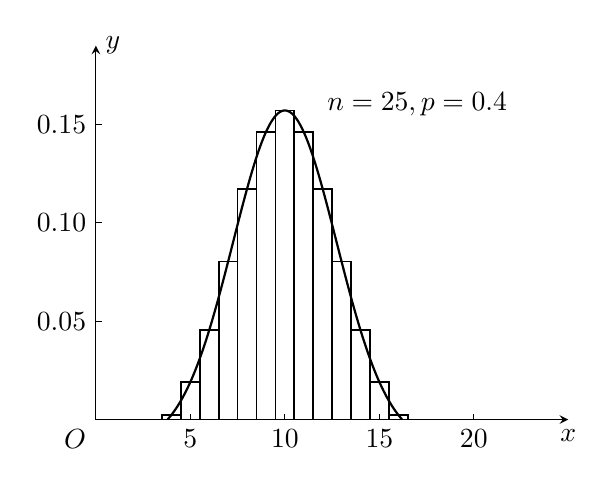
\begin{tikzpicture}[>=stealth,xscale=0.24,yscale=25]
        \draw[->](0,0)node[below left]{$O$}--(25,0)node[below]{$x$};
        \draw[->](0,0)--(0,0.19)node[right]{$y$};
        \foreach \x in {5,10,15,20} \draw (\x,0) node [below] {$\x$} -- (\x,0.003);
        \foreach \x in {0.05,0.10,0.15} \draw (0,\x) node [left] {$\x$} -- (0.3,\x);
        \draw[samples=150,domain=3.8:16.2,thick] plot(\x,{0.17*e^(-(\x-10)^2/15)-0.013});
        \foreach \x in {4,5,...,16} \draw[semithick] (\x-0.5,0) -- (\x-0.5,{0.17*e^(-(\x-10)^2/15)-0.013}) -- (\x+0.5,{0.17*e^(-(\x-10)^2/15)-0.013}) -- (\x+0.5,0) -- cycle;
        \node at (17,0.16) {$n=25,p=0.4$};
    \end{tikzpicture}
    \caption{二项分布正态近似时的修正}\label{fig:4.4.2}
\end{figure}

下面在给出棣莫弗-拉普拉斯极限定理定理的应用之前, 先说明两点:
\begin{enumerate}
    \item 因为二项分布是离散分布, 而正态分布是连续分布, 所以用正态分布作为二项分布的近似计算中, 作些修正可以提高精度.
    若 $ k_1 < k_2 $ 均为整数, 一般先作如下修正后再用正态近似 $ P ( k_1 \leq \mu_n \leq k_2) = P ( k_1 - 0.6 < \mu_n < k_2 + 0.5 ) $.

    譬如 $ \mu_n \sim b (25, 0.4) $, $ P ( 5 \leq \mu_n \leq 15) $ 的值为图~\ref{fig:4.4.2} 中长条矩形的面积, 其精确值为 \num{0.9780}.

    使用修正的正态近似
    \begin{align*}
        P ( 5 \leq \mu_n \leq 15) & = P ( 5 - 0.5 < \mu_n < 15 + 0.5 )\\
        & \sim \Phi \biggl( \frac{15 + 0.5 -10}{\sqrt{6}} \biggr) - \Phi \biggl( \frac{5 - 0.5 - 10}{\sqrt{6}} \biggr)\\
        & = 2 \Phi (2.245) - 1 = 0.9754.
    \end{align*}
    不用修正的正态近似
    \begin{align*}
        P ( 5 \leq \mu_n \leq 15) & \sim \Phi \biggl( \frac{15 -10}{\sqrt{6}} \biggr) - \Phi \biggl( frac{5 - 10}{\sqrt{6}} \biggr)\\
        & = 2 \Phi (2.041) - 1 = 0.9588.
    \end{align*}
    可见不用修正的正态近似误差较大.

    \item 若记 $ \beta = \Phi (y) $, 则由棣莫弗-拉普拉斯极限定理给出的近似式
    \begin{equation*}
        P \bigl( Y_n^* \leq y \bigr) \sim \Phi (y) = \beta,
    \end{equation*}
    可用来解决三类计算问题:
    \begin{enumerate}
        \item 已知 $n$, $y$ 求 $\beta$,
        \item 已知 $n$, $\beta$ 求 $y$,
        \item 已知 $y$, $\beta$ 求 $n$,
    \end{enumerate}
\end{enumerate}

以下我们就分这三类情况给出一些具体的例子.

\subsubsection{给定 $n$, $y$ 求 $\beta$}

\begin{example}\label{exam:4.4.5}
    一复杂系统由100个相互独立工作的部件组成, 每个部件正常工作的概率为 0.9.
    已知整个系统中至少有 85 个部件正常工作, 系统工作才正常.
    试求系统正常工作的概率.
\end{example}

\begin{solution}
    记 $ n = 100 $, $ Y_n $ 为 100 个部件中正常工作的部件数, 则
    \begin{equation*}
        Y_n \sim b (100, 0.9), \ E \bigl( Y_n \bigr) = 90, \\Var  \bigl( Y_n \bigr) = 9.
    \end{equation*}
    所求概率为
    \begin{align*}
        P \bigl( Y_n \geq 85 \bigr) & \sim 1 - \Phi \biggl( \frac{85 - 0.5 - 90}{3} \biggr)\\
        & = 1 - \Phi \biggl( - \frac{5.5}{3} \biggr)
        = \Phi (1.83) = 0.966.
    \end{align*}
\end{solution}

\begin{example}\label{exam:4.4.6}
    某药厂生产的某种药品, 声称对某疾病的治愈率为 \SI{80}{\percent}.
    现为了检验此治愈率, 住意抽取 100 个此种病患者进行临床试验, 如果有多于 75 人治愈, 则此药通过检验.
    试在以下两种情况下, 分别计算此药通过检验的可能性.
    \begin{enumerate}
        \item 此药的实际治愈率为 \SI{80}{\percent},
        \item 此药的实际治愈率为 \SI{70}{\percent}
    \end{enumerate}
\end{example}

\begin{solution}
    记 $ n = 100 $, $ Y_n $ 为 100 个临床受试者中的治愈者人数.
    \begin{enumerate}
        \item 因为 $ Y_n \sim b (100, 0.8) $, $ E (Y_n) = 80 $, $\Var  (Y_n) = 16 $.
        所以通过检验的可能性为
        \begin{align*}
            P \bigl( Y_n > 75 \bigr) & \sim 1 - \Phi \biggl(\frac{75 - 0.5 - 80}{4} \biggr)\\
            & = 1 - \Phi \biggl( -\frac{5.5}{4} \biggr)
            = \Phi (1.375) = 0.9155.
        \end{align*}
        即此药通过检验的可能性是较大的.

        \item 因为 $ Y_n \sim b (100, 0.7) $, $ E (Y_n) = 70 $, $\Var  (Y_n) = 21 $.
        所以通过检验的可能性为
        \begin{align*}
            P \bigl( Y_n > 75 \bigr) & \sim 1 - \Phi \biggl(\frac{75 - 0.5 - 70}{\sqrt{21}} \biggr)\\
            & = 1 - \Phi ( 0.982 )
            = 1-0.8370 = 0.1630.
        \end{align*}
        即此药通过检验的可能性是很小的.
    \end{enumerate}
\end{solution}

\subsubsection{给定$n$, $\beta$ 求 $y$}

\begin{example}\label{exam:4.4.7}
    某车间有同型号的机床 200 台, 在一小时内每台机床约有 \SI{70}{\percent} 的时间是工作的.
    假定各机床工作是相互独立的, 工作时每台机床要消耗电能 \SI{15}{\kilo\watt}.
    问至少要多少电能, 才可以有 \SI{95}{\percent} 的可能性保证此车间正常生产.
\end{example}

\begin{solution}
    记 $ n = 200 $, $ Y_n $ 为 200 台机床中同时工作的机床数, 则 $ Y_n \sim b (200,0.7) $, $ E ( Y_n ) = 140 $, $\Var  (Y_n) = 42 $.

    因为 $ Y_n $ 台机床同时工作需消耗 $ 15Y_n $ (\si{\kilo\watt}) 电能, 所以设供电数为 $ y $ (\si{\kilo\watt}), 则正常生产为 $\{ 15 Y_n \leq y \}$, 由题设 $ P ( 15Y_n \leq y ) \geq 0.95 $, 其中
    \begin{equation*}
        P \bigl( 15Y_n \leq y \bigr) \approx \Phi \left( \frac{y/15 + 0.5 - 140}{\sqrt{42}} \right) \geq 0.95.
    \end{equation*}
    查正态分布表得
    \begin{equation*}
        \frac{y/15 + 0.5 - 140}{\sqrt{42}} \geq 1.645.
    \end{equation*}
    从中解得 $ y \geq $ \SI{2252}{(\kilo\watt)}, 即此车间每小时至少需要 \SI{2252}{(\kilo\watt)} 电能, 才有 \SI{95}{\percent} 的可能性保证此车间正常生产.
\end{solution}

\subsubsection{给定 $y$, $\beta$ 求 $n$}

\begin{example}\label{exam:4.4.8}
    某调查公司受委托, 调查某电视节目在 S 市的收视率 $ p $, 调查公司将所有调查对象中收看此节目的额率作为 $ p $的估计 $ \hat{p} $.
    现在要保证有 \SI{90}{\percent} 的把握, 使得调查所得收视率 $ \hat{p} $ 与真实收视率 $p$ 之间的差异不大于 \SI{5}{\percent}.
    问至少要调查多少对象?
\end{example}

\begin{solution}
    设共调查 $n$ 个对象, 记
    \begin{equation*}
        X_i =
        \begin{cases}
            1, & \text{第} \ i \ \text{个调查对象收看此电视节目},\\
            0, & \text{第} \ i \ \text{个调查对象不看此电视节目},
        \end{cases}
    \end{equation*}
    则 $ X_i $ 独立同分布, 且 $ P (X_i = 1) = p $, $ P (X_i = 0) = 1 - p $, $ i =1, 2, \dotsc, n $.
    又记 $ n $ 个被调查对象中, 收看此电视节目的人数为 $ Y_n $, 则有
    \begin{equation*}
        Y_n = \sum_{i=1}^n X_i \sim b (n, p).
    \end{equation*}
    由大数定律知, 当 $ n $ 很大时, 频率 $ Y_n / n $ 与概率 $ p $ 很接近, 即用频率作为 $ p $ 的估计是合适的.
    根据题意有
    \begin{equation*}
        P \biggl( \biggl\lvert \frac{1}{n} \sum_{i=1}^n X_i - p \biggr\rvert < 0.05 \biggr)
        \approx 2 \Phi \biggl( 0.05 \sqrt{\frac{n}{p (1 - p)}} \biggr) - 1
        \geq 0.90.
    \end{equation*}
    所以
    \begin{equation*}
        \Phi \biggl( 0.05 \sqrt{\frac{n}{p (1 - p)}} \biggr) \geq 0.95.
    \end{equation*}
    查正态分布表得
    \begin{equation*}
        0.05 \sqrt{\frac{n}{p (1 - p)}} \geq 1.645.
    \end{equation*}
    从中解得
    \begin{equation*}
        n \geq p (1 - p) \frac{1.645^2}{0.05^2} = p (1 - p) \times 1082.41.
    \end{equation*}
    又因为 $ p (1-p) \leq 0.25 $, 所以 $ n \geq 270.6 $, 即至少调查271个对象.
\end{solution}

\subsection{独立不同分布下的中心极限定理}

前面我们已经在独立同分布的条件下, 解决了随机变量和的极限分布问题.
在实际间题中说诸 $ X_i $ 具有独立性是常见的, 但是很难说诸 $ X_i $ 是``同分布''的随机变量.
正如前面所提到的测量误差 $ Y_n $ 的产生是由大量``微小的''相互独立的随机因素叠加而成的, 即 $ Y_n = \sum_{i=1}^n X_i $, 则诸 $ X_i $ 间具有独立性, 但不一定同分布.
本节研究独立不同分布随机变量和的极限分布问题, 目的是给出极限分布为正态分布的条件.

为使极限分布是正态分布, 必须对 $ Y_n = \sum{i=1}^n X_i $ 的各项有一定的要求.
譬如若允许从第二项起都等于0, 则极限分布显然出 $ X_1 $ 的分布完全确定, 这时就很难得到什么有意思的结果.
这就告诉我们, 要使中心极限定理成立, 在和的各项中不应有起突出作用的项, 或者说, 要求各项在概率意义下``均匀地小''.
下面我们来分析如何从数学式子上明确表达这个要求.

设 $ \{ X_n \} $ 是一个相互独立的随机变量序列, 它们具有有限的数学期望和方差:
\begin{equation*}
    E \bigl( X_i \bigr) \mu_i, \;\Var  \bigl( X_i \bigr) = \sigma_i^2, \; i = 1, 2, \dotsc.
\end{equation*}

要讨论随机变量的和 $ Y_n = \sum{i=1}^n X_i $, 我们先将其标准化, 即将它减去均值、除以标准差, 由于
\begin{align*}
    E \bigl( Y_n \bigr) & = \mu_1 + \mu_2 + \dotsb + \mu_n,\\
    \sigma \bigl( T_n \bigr) & = \sqrt{Var \bigl( X_i \bigr)} = \sqrt{\sigma_1^2 + \sigma_2^2 + \dotsb + \sigma_n^2},
\end{align*}
且记 $ \sigma ( Y_n ) = B $, 则 $ Y_n $ 的标准化为
\begin{equation*}
    Y_n^* = \frac{Y_n - \bigl( \mu_1 + \mu_2 + \dotsb + \mu_n \bigr)}{B_n} = \sum_{i=1}^n \frac{X_i - \mu_i}{B_n}.
\end{equation*}

如果要求 $ Y_n^* $ 中各项 $ (X_i - \mu_i) / B_n $ ``均匀地小'', 即对任意的 $ \tau > 0 $, 要求事件
\begin{equation*}
    A_k = \left\{ \frac{\lvert X_i - \mu_i \rvert}{B_n} > \tau \right\} = \bigl\{ \lvert X_i - \mu_i \rvert > \tau B_n \bigr\}
\end{equation*}
发生的可能性小, 或直接要求其概率趋于0.
为达到这个目的, 我们要求
\begin{equation*}
    \lim_{n \to +\infty} P \left\{ \max_{1 \leq i \leq n} \lvert X_i - \mu_i \rvert > \tau B_n \right\} = 0.
\end{equation*}
因为
\begin{align*}
    P \left\{ \max_{1 \leq i \leq n} \lvert X_i - \mu_i \rvert > \tau B_n \right\} & = P \left\{ \cup_{i=1}^n \bigl( \lvert X_i - \mu_i \rvert > \tau B_n \bigr) \right\}\\
    & \leq \sum_{i=1}^n P \bigl( \lvert X_i - \mu_i \rvert > \tau B_n \bigr).
\end{align*}
若设诸 $ X_i $ 为连续随机变量, 其密度函数为 $ p_i (x) $, 则
\begin{align*}
    \text{上式} & = \sum_{i=1}^n \int_{\lvert x - \mu_i \rvert > \tau B_n} p_i (x) \dd x\\
    & \leq \frac{1}{\tau^2 B_n^2} \sum_{i=1}^n \int_{\lvert x - \mu_i \rvert > \tau B_n} \bigl( x - \mu_i \bigr)^2 p_i (x) \dd x.
\end{align*}
因此, 只要对任意的 $ \tau > 0 $, 有
\begin{equation}\label{eq:4.4.4}
    \lim_{n \to +\infty} \frac{1}{\tau^2 B_n^2} \sum_{i=1}^n \int_{\lvert x - \mu_i \rvert > \tau B_n} \bigl( x - \mu_i \bigr)^2 p_i (x) \dd x = 0
\end{equation}
就可保证 $ Y_n^* $ 中各加项``均匀地小''.

上述条件 \eqref{eq:4.4.4} 称为{\heiti 林德贝格条件}\index{林德贝格条件}.
林德贝格证明了满足 \eqref{eq:4.4.4} 条件的和 $ Y_n $ 的极限分布是正态分布, 这就是下面的给出的{\heiti 林德贝格中心极限定理}\index{林德贝格中心极限定理}, 由于这个定理的证明需要更多的数学工具, 所以以下仅叙述定理, 略去其证明.

\begin{theorem}{林德贝格中心极限定理}{4.4.3}
    设独立随机变量序列 $ \{ X_n \} $ 满足林德贝格条件, 则对任意的x, 有
    \begin{equation*}
        \lim_{n \to +\infty} P \left\{ \frac{1}{B_n} \sum_{i=1}^n \bigl( X_i - \mu_i \bigr) \leq x \right\} = \frac{1}{\sqrt{2\pi}} \int_{-\infty}^x \ee^{-t^2 /2 } \dd t.
    \end{equation*}
\end{theorem}

假如独立随机变量序列 $ \{ X_n \} $ 具有同分布和方差有限的条件, 则必定满足以上 \eqref{eq:4.4.4} 林德贝格条件, 也就是说定理~\ref{thm:4.4.1} 是定理~\ref{thm:4.4.3} 的特例.
这一点是很容易证明的:

设 $ \{ X_n \} $ 是独立同分布随机变量序列, 为确定起见, 设诸 $ X_n $ 是连续随机变量, 其共同的密度函数为 $ p (x) $, $ \mu_i = \mu $, $ \sigma_i = \sigma $.
这时 $ B_n = \sigma \sqrt{\mu} $, 由此得
\begin{equation*}
    \frac{1}{B_n^2} \sum_{i=1}^n \int_{\lvert x - \mu_i \rvert > \tau B_n} ( x - \mu_i )^2 p (x) \dd x = \frac{n}{n \sigma^2} \int_{\lvert x - \mu \rvert > \tau \sigma \sqrt{n}} ( x - \mu )^2 p (x) \dd x.
\end{equation*}
因为方差存在, 即
\begin{equation*}
   \Var  \bigl( X_i \bigr) = \int_{-\infty}^{+\infty} ( x - \mu )^2 p (x) \dd x < + \infty.
\end{equation*}
所以其尾部积分一定有
\begin{equation*}
    \lim_{n \to +\infty} \int_{\lvert x - \mu \rvert > \tau \sigma \sqrt{n}} ( x - \mu )^2 p (x) \dd x = 0,
\end{equation*}
故林德贝格条件满足.

林德贝格条件虽然比较一般, 但该条件较难验证, 下面的李雅普诺夫条件则比较容易验证, 因为它只对矩提出要求, 因而便于应用.
下面我们仅叙述其结论, 证明从略.

\begin{theorem}{李雅普诺夫中心极限定理}{4.4.4}
    设 $ \{ X_n \} $ 为独立随机变量序列, 若存在 $ \delta > 0 $, 满足
    \begin{equation}\label{eq:4.4.5}
        \lim_{n \to +\infty} \frac{1}{B_n^{2 + \delta}} \sum_{i=1}^n E \bigl( \bigl\lvert X_i - \mu \bigr\rvert^{2+\delta} \bigr) = 0,
    \end{equation}
    则对任意的 $ x $, 有
    \begin{equation*}
        \lim_{n \to +\infty} P \biggl\{ \frac{1}{B_n} \sum_{i=1}^n \bigl( X_i - \mu_i \bigr) \leq x \biggr\} = \frac{1}{\sqrt{2\pi}} \int_{-\infty}^x \ee^{-t^2/2} \dd t,
    \end{equation*}
    其中 $ \mu_i $ 与 $ B_n $ 如前所述.
\end{theorem}

\begin{example}\label{exam:4.4.9}
    一份考卷由 99 个题目组成, 并按由易到难顺序排列, 某学生答对第 1 题的概率为 0.99; 答对第 2 题的概率为 0.98; 一般地, 他答对第 $ i $题的概率为 $ 1 - i/100 $, $ i = 1, 2, \dotsc $.
    假如该学生回答各题目是相互独立的, 并且要正确回答其中 60 个题日以上 (包括 60 个) 才算通过考试.
    试计算该学生通过考试的可能性多大?
\end{example}

\begin{solution}
    设
    \begin{equation*}
        X_i =
        \begin{cases}
            1, & \text{若学生答对第} \ i \text{题},\\
            0, & \text{若学生答错第} \ i \text{题}.
        \end{cases}
    \end{equation*}
    于是 $ X_i $ 相互独立, 且服从不同的二点分布:
    \begin{equation*}
        P \bigl( X_i = 1 \bigr) = p_i = 1 - \frac{i}{100}, \
        P \bigl( X_i = 0 \bigr) = 1 - p_i = \frac{i}{100}, \
        i = 1,2, \dotsc, 99.
    \end{equation*}
    而我们要求的是
    \begin{equation*}
        P \biggl( \sum_{i=1}^99 X_i \geq 60 \biggr).
    \end{equation*}

    为使用中心极限定理, 我们可以设想从 $ X_{100} $ 开始的随机变量都与 $ X_{99} $ 同分布, 且相互独立.
    下面我们用 $ \delta = 1 $ 来验证随机变量序列 $ \{ X_n \} $ 满足李雅普诺夫条件 \eqref{eq:4.4.5}, 因为
    \begin{align*}
        & B_n = \sqrt{\sum_{i=1}^n\Var  \bigl( X_i \bigr)} = \sqrt{\sum_{i=1}^n p_i \bigl( 1 - p_i \bigr)} \to +\infty, \ n \to +\infty\\
        & E \bigl( \bigl\lvert X_i - p_i \bigr\rvert^3 \bigr) \bigl( 1 - p_i \bigr)^3 p_i + p_i^3 \bigl( 1 - p_i \bigr) \leq p_i \bigl( 1 - p_i \bigr),
    \end{align*}
    于是
    \begin{equation*}
        \frac{1}{B_n^3} \sum_{i=1}^n E \bigl( \bigl\lvert X_i - p_i \bigr\rvert^3 \bigr) \leq \frac{1}{\bigl( \sum_{i=1}^n p_i ( 1 - p_i ) \bigr)^{1/2}} \to 0, \ n \to +\infty.
    \end{equation*}
    即 $ \{ X_n \} $ 满足李雅普诺夫条件 \eqref{eq:4.4.5}, 所以可以使用中心极限定理.
    又因为
    \begin{align*}
        & E \Biggl( \sum_{i=1}^{99} X_i \Biggr) = \sum_{i=1}^{99} p_i = \sum_{i=1}^{99} \biggl( 1 - \frac{i}{100} \biggr) = 49.5\\
        & B_{99}^2 = \sum_{i=1}^{99}\Var  \bigl( X_i \bigr) = \sum_{i=1}^{99} \biggl( 1 - \frac{i}{100} \biggr) \biggl( \frac{i}{100} \biggr) = 16.665.
    \end{align*}
    所以该学生通过考试的可能性为
    \begin{align*}
        P \Biggl( \sum_{i=1}^{99} X_i \geq 60 \Biggr) & = P \left( \frac{\sum_{i=1}^{99} X_i - 49.5}{\sqrt{16.665}} \geq \frac{60-49.5}{\sqrt{16.665}} \right)\\
        & \approx 1 - \Phi (2.5735) = 0.005.
    \end{align*}
    由此看出: 此学生通过考试的可能性很小, 大约只有千分之五.
\end{solution}

\begin{xiti}
    \item 某保险公司多年的统计资料表明, 在索赔户中被森素赔户占 \SI{20}{\percent}, 以 $ X $ 表示在随意抽查的 \num{100} 个家赔户中因被盗向保险公司素赔的户数.
    \begin{enumerate}
        \item 写出 $X$ 的分布列,
        \item 求被盗索赔户不少于 14 户且不多于 30 户的概率的近似值.
    \end{enumerate}
    \item 某电于计算机主机有 \num{100} 个终端, 每个终端有 \SI{80}{\percent} 的时间被使用.
    若各个终端是否被使用是相互独立的, 试求至少有15个终端空闲的概率.
    \item 有一批建筑房屋用的木柱, 其中 \SI{80}{\percent} 的长度不小于 \SI{3}{\meter}, 现从这批木柱中随机地取出 \num{100} 根, 问其中至少有 30 根短于 \SI{3}{\meter} 的概率是多少?
    \item 掷一颗散子 100 次, 记第 $ i $ 次挪出的点数为 $ X_i $, $ i = 1, 2, \dotsc, 100 $, 点数之平均为 $ \bar{X} = \frac{1}{n} \sum_{i=1}^{100} X_i $.
    试求薇率 $ P (3 \leq \bar{X} \leq 4 )$.
    \item 设 $ X_1, X_2, \dotsc, X_{48} $ 为独立同分布的随机变量, 共同分布为 $ U (0,5) $.
    其算术平均为 $ \bar{X} = \frac{1}{n} \sum_{i=1}^{48} X_i $, 试求概率 $ P (2 \leq \bar{X} \leq 3) $.
    \item 某汽车销售点每天出售的汽车数服从参数为 $ \lambda = 2 $ 的泊松分布.
    若一年 365 天都经营汽车销售, 且每天出修的汽车数是相互独立的, 求一年中售出 700 辆以上汽车的概率.
    \item 某餐厅每天接待 400 名顾客, 设每位顾客的消费额 (元) 服从 $ (20, 100) $ 上的均匀分布, 且顾客的消费额是相互独立的.
    试求:
    \begin{enumerate}
        \item 该餐厅每天的平均营业额,
        \item 该餐厅每天的营业额在平均营业额 $ \pm 760 $ 元内的概率.
    \end{enumerate}
    \item 一仪器同时收到 50 个信号 $ U_i $, $ i = 1, 2, \dotsc, 50 $.
    设 $ U_i $ 是相互猫立的, 且都服从 $ (0, 10) $ 内的均匀分布, 试求 $ P ( \sum_{i=1}^{50} U_i > 300) $.
    \item 计算机在进行加法运算时对每个加数取整数 (取最为接近于它的整数).
    设所有的取整误差是相互独立的, 且它们都服从 $ (-0.5, 0.5) $ 上的均匀分布.
    \begin{enumerate}
        \item 若将 \num{1500} 个数相加, 求误差总和的绝对值超过 15 的概率,
        \item 最多几个数加在一起可使得误差总和的绝对值小于 10 的概率不小于 \SI{95}{\percent}.
    \end{enumerate}
    \item 设各零件的重量都是随机变量, 它们相互独立, 且服从相同的分布, 其数学期望为 \SI{0.5}{\kg}, 标准差为 \SI{0.1}{\kg}, 问 \num{5000} 只零件的总重量超过 \SI{2510}{\kg} 的概率是多少?
    \item 某种产品由 20 个相同部件连接而成, 每个部件的长度是均值为 \SI{2}{\mm}、标准差为 \SI{0.02}{\mm} 的随机变量.
    假如这 20 个部件的长度相互独立同分布, 且规定产品总长为 \SI{40}{\mm}$\pm$\SI{0.2}{\mm} 时为合格品, 求该产品的不合格品率.
    \item 进行独立重复试验, 每次试验中事件 A 发生的概率为 0.25.
    试问能以 \SI{95}{\percent} 的把握保近 \num{1000} 次试验中事件 A 发生的频率与概率相差多少?
    此时 A 发生的次数在什么范围内?
    \item 设某生产线上组装每件产品的时间服从指数分布, 平均需要 \SI{10}{\minute}, 且各件产品的组装时间是相互独立的.
    \begin{enumerate}
        \item 试求组装 100 件产品需要 \SI{15}{\hour} 至 \SI{20}{\hour} 的概率,
        \item 保证有 \SI{95}{\percent} 的可能性, 问 \SI{16}{\hour} 内最多可以组装多少件产品.
    \end{enumerate}
    \item 某种福利彩票的奖金额 $X$ 由摇奖决定, 其分布列为

    \begin{tabularx}{0.95\linewidth}{>{\centering\arraybackslash}X|*{7}{>{\centering\arraybackslash}X}}
        \toprule
        $X$ (万元) & 5 & 10 & 20 & 30 & 40 & 50 & 100\\
        \midrule
        $P$ & 0.2 & 0.2 & 0.2 & 0.1 & 0.1 & 0.1 & 0.1\\
        \bottomrule
    \end{tabularx}

    若一年中要开出 300 个奖, 问需要多少奖金总额, 才有 \SI{95}{\percent} 的把握能够发放奖金.
    \item 一家有 500 间客房的大旅馆的每间客房装有一台 \SI{2}{\kilo\watt} 的空调机.
    若开房率为 \SI{80}{\percent}, 需要多少 \si{\kilo\watt} 的电力才能有 \SI{99}{\percent} 的可能性保证有足够的电力使用空调机.
    \item 独立重复地对某物体的长度 $a$ 进行 $n$ 次测量, 设各次测量结果 $ X_i $ 跟从正态分布 $ N (a, 0.2^2) $.
    记 $ \bar{X} $ 为 $a$ 次测量结果的算术平均值, 为保证有 \SI{95}{\percent} 的把握使平均值与实际值 $a$ 的差异小于 0.1, 问至少需要测量多少次?
    \item 某工厂每月生产 \num{10000} 台液晶投影机, 但它的液晶片车间生产液晶片合格品率为 \SI{80}{\percent}, 为了以 \SI{99.7}{\percent} 的可能性保证出厂的液晶投影机都能装上合格的液晶片, 试问该液晶片车间每月至少应该生产多少片液晶片?
    \item 某产品的合格品率为 \SI{99}{\percent}, 问包装箱中应该装多少个此种产品, 才能有 \SI{95}{\percent} 的可能性使每箱中至少有 100 个合格产品.
    \item 为确定某城市成年男子中吸烟者的比例 $p$, 任意调查 $n$ 个成年男子, 记其中的吸烟人数为 $m$, 问 $n$ 至少为多大才能保证 $m/n $与 $ p $的差异小于 0.01 的概率大于 \SI{95}{\percent}.
\end{xiti}
